\chapter{Literature Review}
\label{literatureReview}

\section{Wireless Sensor Networks}
A WSN is a network of sensor nodes that are used to collect data from the target area over the radio. These data that the sensors send can be normal data packets or sensor measurements data such as the temperature and movement in the specific area where the sensors are located. The sensors can be used for continuous sensing, event detection, location sensing and local control of actuators to control different components in the sensing device, such as adjusting the sensor parameters or move the sensor if it is a mobile sensor.

This chapter describes the available WSN applications, challenges and known issues that occur in WSNs. Many previous studies were done in order to maximise the lifetime of sensor networks while keeping the energy to a minimum. This chapter also briefly describes the existing solutions for energy efficient multi channel at the MAC and network layers which prompted to the work of MCRP. 

\subsection{Applications Overview}
There are five types of deployed WSNs: terrestrial WSNs, underground WSNs, underwater WSNs, multimedia WSNs and mobile WSNs which cover different types of environment; to deploy on land, underground and water \cite{wsnSurvey1}. Unlike other sensor nodes, multimedia WSNs have the ability to monitor and track events in the form of video and audio as they are equipped with cameras and microphones for multi-media data which can enhance the existing WSN applications \cite{wsnSurvey3}. Mobile WSNs on the other hand, can be any type of sensors that have the capability to reposition and organise itself in the network.

WSNs evolution is driven by a number of emerging applications that focuses on the importance of wireless sensors in applications such as smart grid, areas in smart cities, and automated home, building and industrial applications \cite{beyondInteroperability}. Smart grid could save considerable amounts of energy by improving the existing electrical grid power. Smart cities which includes automated home, building and industrial in populated cities can improve the environment quality by allowing automated services such as pollution monitoring and automated energy control (temperature and lighting) which increases the energy saving in the process. 

WSNs applications are important as sensor nodes can be easily deployed at all types of environment, installed and require minimal maintenance for a period of time. The main challenges in these applications are in term of reliable event detection, securing high data rates for efficient data routing and dense or sparse nodes deployment.

WSNs applications can be categorised into five main monitoring and tracking applications which are the environmental applications, health applications, home applications, military applications and other commercial applications \cite{wsnSurvey2}. These applications are briefly described in the next section with examples for each category. 

\subsubsection{Environmental Applications}
The environment applications can be divided into two types; tracking and monitoring. The tracking applications are used to record the movements of animals such as birds, insects and small animals at a certain area. Monitoring applications are used to monitor the environment conditions such as forest fire detection, flood detection, biocomplexity mapping \cite{Cerpahabitatmonitoring}, precision agriculture monitoring and volcanic monitoring \cite{volcano}.

In forest fire detection, the sensor nodes are used to relay the exact originated location of the fire to the end users to control it from spreading. ALERT is an example of a flood detection system that is deployed in the United States. ALERT consists of several types of sensors such as rainfall, water level and weather sensors. In agriculture, the sensor nodes are used to monitor the level of pesticides in drinking water, soil erosion and air pollution in real time. In volcanic monitoring, the sensor nodes allow measurements to be taken from locations that are otherwise inaccessible. 

\subsubsection{Health Applications}
Sensor networks in health applications can be used to monitor human physiological data such as detecting elderly people's behaviour in case of a fall, drug administration \cite{telemonitoring} in hospitals to minimise incorrect prescription of medication to patients, and to monitor and track doctors and patients locations in a hospital. Examples of these are \textit{telecare} and \textit{telehealth} \cite{telehealth}.

Telecare is a system of wireless sensors that are placed around the house and can be a personal alarm in form of a small wristband or pendant. These sensors can detect risks such as a fall, motion sensor that turns on the lights at night when someone get out of bed, a pressure mat on the mattress to sense if someone gets back to bed or a sensor on the door in case it is not closed, are a few examples of the system. If a risk is detected, it sends the alert immediately for attention to a telecare monitoring centre. 

Telehealth is a small equipment to monitor health from home. It can be used to measure the blood pressure, blood glucose levels, oxygen levels, weight or temperature. The measurements are automatically transmitted to a monitoring centre. The healthcare professional will be contacted if the information raised an alarm for actions to be taken. 

\subsubsection{Home Applications}
In home automation \cite{homeautomation}, the smart sensor nodes and actuators can be buried in the appliances such as vacuum cleaners, microwave ovens and refrigerators which allows them to form an interaction through the Internet. Some of the recent home automation are \textit{Samsung SmartThings} and \textit{Nest Thermostat}.

Samsung SmartThings allows devices at home to be monitored and controlled from a mobile phone such as controlling the thermostats and lighting. Nest Thermostat is a self-learning thermostat that is consists of activity sensors, temperature sensors, humidity sensor and a Wi-Fi radio. These sensors allow Nest to learn the heating and cooling habits which allows it to shuts down due to inactivity to conserve the energy. Nest is weather aware. It uses its Wi-Fi connection to get the weather condition and forecasts, and integrate the information to understand the affects of the outside temperature to the energy usage. Nest is also able to connect with other appliances that are Nest supported. The appliances can automatically start without any need to program it as it learns from other devices.

\subsubsection{Military Applications}
WSNs are used in military applications to monitor friendly forces, equipments and ammunitions by attaching sensors which report the status back to the base station; battlefield surveillance by covering critical terrains, routes, paths and straits with sensors and reconnaissance the opposing forces; assess battle damage, and to detect nuclear, biological and chemical attack by deploying sensors to explore areas and serve as warning systems to avoid casualties.

An example of military application is \textit{PinPtr} \cite{Simonpinptr}. PinPtr is an experimental counter-sniper system. It was developed to detect and locate shooters by measuring shot time of arrival of the muzzle blasts and shock waves from the sensors that are densely deployed. The measurements are routed to the base station where the shooter's location is computed. PinPtr was demonstrated and evaluated in realistic urban environment from various US Army test facilities.

\subsubsection{Other Commercial Applications}
Other available commercial applications are environmental control in office buildings such as controlling the air flow and temperature for different part of the building; car thefts monitoring and detection within specific region; inventory control management to track and locate the inventories in the warehouses; machine diagnosis in order to predict equipment failure for maintenance through vibration signatures gathered by sensors \cite{industrialsensor}; and vehicle tracking and detection for parking purposes such as the \textit{Smart Parking} from \textit{Streetline} and \textit{SmartPark}. 

Smart Parking solutions are used in more than 40 cities and universities in North America and Europe. The system could make intelligent decisions using the data from the real time and historical analytical reports to improve the parking ecosystem. The system detects vehicle occupancy in real time which simplifies the parking experience by guiding drivers to the available spaces. It can also guide officers to unpaid violations and overstays as the arrival and departure times are recorded; and to detect if a car is parked over the no parking and restricted zones. 

SmartPark is a parking solution in the UK, currently operating in Birmingham and in the central London Borough of Westminster. These applications enable drivers to find vacant space within the busy town and city centres quicker.

\subsection{WSN Challenges and Issues}
WSNs are widely used in various kinds of applications. This is because sensor nodes can be densely deployed, easy to install and require minimal maintenance over a period of time. However, WSNs suffer from limited hardware resources which only allow limited computational functionalities to be performed. It also suffers from limited energy capacities as the sensors are battery powered and they will become faulty and not able to function once the certain threshold of energy level is reached. It also operates in an unreliable radio environment that is noisy and error prone which drain the sensors batteries at a higher rate.

These constraints have a major impact on the sensors performance. In order to prolong the sensors lifetime thus, the network lifetime, the sensors need to be able to cope with the limitations and be as energy-efficient as possible to guarantee good overall performance.

\section{Maximising Lifetime and Minimising Energy}
In WSNs, it is necessary to estimate the nodes power consumption before they are deployed to enable accurate forecast of the energy consumption. The estimations are used to determine the nodes lifetime before maintenance and batteries replacements are required in order to have a functional network. Unfortunately, the node lifetime is very dependent on the radio environment that can be unstable, noisy and error prone which makes energy consumption to vary \cite{alexlifetime}. The network lifetime, however, depends on various factors such as the network architecture and protocols, channel characteristics, energy consumption model and the network lifetime definition. In order to increase the network lifetime, these information regarding the channel and residual energy of the sensors should be exploited.

There are various definitions of network lifetime that have been used. These definitions are application-specific as some applications might tolerate a considerable number of loss nodes, while some applications require a higher number of nodes which any loss is considered critical to the network such as in sparsely deployed nodes of an area. The definitions impact the performance differently, depending on the applications. The various definitions are:

\begin{itemize}
\item \textbf{The first node to die} - The network lifetime is defined as the first node to fail in the network \cite{maxmin, erapl}. In \cite{lifetimedef1}, the simulation ends when a node reaches the energy level of zero.

\item \textbf{The number of alive nodes} - The network lifetime is the number of remaining nodes as a function of time. The network has a longer lifetime with a higher number of remaining nodes \cite{lifetimedef2, smecn}.

\item \textbf{The number of nodes still connected to the sink} - The network is alive based on the remaining number of nodes to have coverage to connect to the sink \cite{smecn}.

\item \textbf{The fraction of alive nodes} - The network lifetime is defined by the percentage of surviving nodes above a threshold.

\item \textbf{Packet delivery ratio} - The network lifetime ends when the packet delivery ratio drops dramatically. GAF \cite{gaf} uses this definition where it is possible when the traffic is kept constant.

\item \textbf{The first failure in data transmission} - The sensor does not have enough energy for transmission \cite{maxmin}.
\end{itemize}


Network lifetime is strongly related to the remaining energy of all nodes. However, maximising the minimal energy of all the nodes is not the best way to prolong the network lifetime as it will place heavy burden to the key nodes such that nodes that are close to the sink. These nodes drain their batteries quicker than other nodes which as a result, shorten the network lifetime.

There are four ways that have been explored from many studies to maximise the network lifetime, which are by introducing (i) energy efficient MAC protocols, (ii) energy efficient routing protocols, (iii) controlling the transmission power and (iv) using energy harvesting. These options are described in details in the next few sections, introducing the differences and advantages, and the existing proposed solutions.

The aim of the WSN design is to extend the network lifetime under the given energy and node constraints without jeopardizing reliability and communications efficiency of the network.

\subsection{MAC Protocols}
Many energy efficient MAC protocols have been proposed to prolong the network lifetime. The radio module that is controlled by the MAC protocol is the major energy consumer in WSNs. The radio uses nearly the same energy in all active operation modes such as the transmit, receive and idle modes \cite{alexlifetime}. Thus, it is important to reduce the radio usage to conserve the nodes energy.

The main causes of energy consumption are nodes collision, overhearing and idle listening \cite{macsurvey, pwmac}. Collision happens when nodes that is within each other transmission range transmits simultaneously. The energy used in the collided transmissions is wasted as none of the nodes would receive the transmitted packet. Multi channel is one of the solutions to overcome collision. Overhearing happens when a node receives irrelevant packets or signals that are not intended to the node. As the radio uses nearly the same energy for all operations, this drains the node energy unnecessarily. In idle listening, the node keeps its radio on while listening to the channel for potential packets. The node does not know when it will be the receiver of the packet. Considerable amounts of energy are wasted as the node keeps its radio on for a longer period listening to an idle channel when it does not receive or transmit packets. 

A vast number of energy efficient MAC protocols have been developed to overcome these problems through \textit{duty cycling}. Duty cycled MAC protocols allow the node to periodically alters the sleep state and listen state. By lowering the duty cycle, the node sleeps for a longer period instead of being permanently active. However, the node needs to have frequent check interval to avoid deafness problem while keeping overhearing to a minimum. This reduces the energy consumed by idle listening and overhearing.

Many MAC protocols such as YMAC \cite{y-mac} uses duty cycle as the indicator to evaluate the energy efficiency performance. This is because it is difficult to measure the nodes energy consumption. However, there are studies that managed to estimate the energy consumption. This is described in Chapter \ref{energyLoss}.

\subsection{Routing Protocols}
Various energy efficient routing protocols for WSNs have been proposed and developed to ensure efficient packet delivery to the destination. The strategies that are used in routing protocols should ensure minimum energy consumption in order to prolong the lifetime of the network. 

A major issue in WSNs routing protocol is in finding and maintaining the optimal routes that are energy efficient. This is due to the energy constraints and unexpected changes in node status such as node failure or unreachable. This causes the topology to be altered frequently to adapt to the changes. Abrupt topology modification is important to avoid the network from being disconnected which leads to higher rate of packet loss at the involved nodes as the routes are not updated.

There a several routing techniques such as flat, hierarchical and location-based routing protocols that are application dependent. Hierarchical structure, as an example, has a balanced energy structure as the packets are transmitted from the lower layer nodes to the upper layer nodes. These different techniques are explained in detail in Section \ref{routingProtocols}. 

The routes that are formed are based on the routing metric \cite{pantazis} that attempts to transmit the packet to the receiver by selecting the most efficient path that the protocol calculated. The path may be the shortest path, lowest expected transmission count path \cite{mrhof} or path that maximises the network lifetime by considering all nodes remaining energy. However, in order to achieve the best network lifetime, the total energy consumption of the network and the nodes minimal remaining energy should be combined for a better balance in the network \cite{erapl}.

%%%The common practice in networks is to use the shortest routes to transfer the packets. This could result the death of the nodes along the shortest path. Since is a WSN every node has to act as a relay in order to forward the message, if some nodes die sooner, due to lack of energy, it is possible that other nodes will not be able to communicate any more. Hence, the network will get disconnected, the energy consumption is not balanced and the lifetime of the whole network is seriously affected. Therefore, a combination between the shortest path and the extension of the network lifetime is the most suitable routing metrics to be used in WSNs. 

%%%A routing algorithm termed Energy-efficient Routing Algorithm to Prolong Lifetime (ERAPL) is proposed. A data gathering sequence (DGS) used to avoid and eliminate mutual transmission and loop transmission among nodes (node is only allowed to transmit to its neighboring node in forward direction only to avoid loop), is constructed and each node proportionally transmit traffic to the links confined in the DGS. The main task of the ERAPL is to determine the optimal outgoing traffic to maximize the network lifetime for a given WSN. In addition, a mathematical programming model, in which minimal remaining energy of nodes and total energy consumptions are included, is presented to optimized network lifetime. ERAPL is a centralised algorithm and runs at the sink; sink knows the topology of the WSN. Sink inform all the nodes in the WSN of a packet that contains the constructed DGS which guides all the nodes to transmit traffic to their respective neighbors so that mutual transmission among nodes and route loop is avoided and accordingly energy is saved. ERAPL can improve network lifetime while expending energy efficiently by constructing a DGS and finding the optimal outgoing traffic proportions for all the nodes to distribute packets to their respective neighbouring nodes \cite{erapl}. 

\subsection{Transmission Power Control} 
Topology control term has been used to mean two different things in WSNs literature. Several authors define topology control as routing protocol techniques. Another definition of topology control is power control techniques which act on the nodes transmission power level \cite{santitopologycontrol}. Topology control term has been interchangeably used with power control. To avoid confusion, the term power control is used in this thesis.

In power control, a node has control over the transmission range of the node's radio which can be manipulated to benefit the network. The power adjustment approach allows the node to vary the transmission power thus range to form a connected network that minimise the energy incurred in transmission. The nodes collaboratively adjust to find the appropriate transmission power which enables the nodes to transmit at a lower transmission power than at the maximum. However, a sparse network would require a higher transmission power than a dense network to be able to transmit to the nearest node. 

The power control technique eliminates links that are wasting the energy resources by fixing the area of coverage thus routing. This reduces collisions as inefficient links of long distance nodes are discarded. However, the nodes need to change the transmission power to adapt to any area coverage changes in order to modify the routing. 

As the transmission ranges are relatively short, the nodes can simultaneously transmit packet without interfering each other, thus reducing congestion from retransmissions. Although power control improves the network traffic flows, it does not reduce the nodes power consumption as it depends on the radio duty cycle. Power savings due to transmission powers are negligible \cite{macsurvey}.

%%Define topology control as a technique used in wireless ad hoc and sensor networks to reduce energy consumption (which is essential to extend the network operational time) and radio interference (with a positive effect on the network traffic carrying capacity). The goal of topology control is to dynamically change the nodes transmitting range in order to maintain some property of the communication graph (connectivity) while reducing the energy consumed by the node transceivers which is strictly related to the transmitting range. 

\subsection{Energy Harvesting}
As mentioned previously, sensor nodes have limited energy capacities as they are battery powered. However, the number of deployed nodes within the specific area has an effect to the nodes energy usage. In a densely deployed nodes area, short range transmission between the nodes could reduce the energy consumption while a sparsely deployed nodes area have a longer range transmission which require higher energy usage. In the situation where the nodes are not densely deployed, energy harvesting may be an option to increase the nodes energy level.

Energy harvesting is when a node tries to replenish its energy by using other energy sources such as solar cells \cite{wsnheap, reviewharvest}, vibration \cite{gilbert2008comparison}, fuel cells, acoustic noise and a mobile supplier \cite{wsnSurvey1}. Solar cell is the current mature technique to harvest energy from light. There is also work in using robots as mobile energy supplier to deliver energy to nodes. This allows a longer network lifetime as the node has restored its energy. 

However, energy harvesting depends on various environment factors such as light, vibration and heat to be generated and converted to the usable electrical energy. There are also other different powering mechanisms that are available such as rechargeable battery with regular recharging from the sunlight \cite{macsurvey}. 

\section{Multichannel MAC Protocol}
%\section{Multichannel MAC Protocol (Data Link Layer)}
In single channel MAC protocols, nodes are configured to use a single channel throughout the nodes lifetime. Frequency agile MAC protocols on the other hand, allow the nodes to switch to different channels during run time. This is possible as recent radio chips take less than 100$\mu$s to switch to a different channel. The channel switching delay is negligible which attracts multi channels to be used in WSNs. Multi channels have the advantage of an increase in robustness against external and between nodes interference which as a result, improves the network traffic flow.

%Thus considering multi-channel. \cite{singh2010routing}

\subsection{Introduction}
%Multichannel communications has potential benefits for wireless networks that include improved resilience against external interference, reduced latency, enhanced reception rate and increased throughput.

There have been many proposals in multichannel communication which uses the duty cycling technique to alter the nodes sleep and listen states. The duty cycling is an important mechanism that helps reducing the nodes energy consumption. However, adjusting the duty cycle does not solve the interference problem as external interference is unpredictable. Multi channel is a preferable solution to improved resilience against interference.

Existing duty cycled multichannel MAC protocols can be categorised into two types; synchronous and asynchronous systems. These are also referred as reservation-based protocol and contention-based protocol by some authors. A synchronous system is a system that requires a tight time synchronisation between nodes. It uses time-scheduled communication where the network clock needs to be periodically synchronised to compensate for time synchronisation error in order for the nodes not to drift in time \cite{y-mac}. The system requires dependency on the time synchronisation and network topology. The knowledge of the network topology is required to be able to establish a schedule for the nodes to access the channel to communicate with the other nodes.

%Crystal clocks used for general sensor node platforms are typically cheap and inaccurate, all nodes have to communicate periodically in order to compensate for time synchronization errors resulting from clock drift. \cite{y-mac}

Asynchronous system on the other hand, does not require synchronisation and topology knowledge but instead is a sender or receiver initiated communication. The nodes compete to access the channel to transmit such that the node postpones its transmission if it senses that the channel is busy, by sending preamble packets, to avoid interfering with the current transmission. In asynchronous systems the nodes are able to self-configure without time synchronization and this can have advantages. There are many studies done in multichannel for both categories.

Multichannel communications have potential benefits for wireless networks that include improved resilience against external interference, reduced latency, enhanced reception rate and increased throughput. A set of existing multichannel MAC protocols are reviewed and compared, highlighting their features and limitations.

%%%If each nodes has an exclusive send time slot (synchronous/reservation-based protocol - sender-initiated approach)in two-hop neighborhood, collision-free access to the medium is guaranteed. Such a scheme is thus able to reduce energy waste by contention and collisions. However, all nodes must wake up at every time slot so as not to miss incoming messages. This results in energy wastage due to idle listening and overhearing. Therefore, scheduling receivers is more energy efficicnet than scheduling senders under light traffic conditions, because each node samples the medium only in its own receive time slot. The contention level is relatively low since contention among senders which have different destination nodes is eliminated. \cite{y-mac}

%%%The sender-initiated approach, a sender transmits preamble before a packet transmission to notify the receiver of the upcoming packet. With receiver-initiated approach, in contrast, sender preambles are replaced with receiver wakeup beacons. Receiver-initiated wakeup beacons are used to avoid long sender-initiated preambles. However, a larger sender duty cycle due to idle listening until the receiver wakes up. In sender-initiated protocols, a sender often shows much larger duty cycle than a receiver, transmitting the preamble until the receiver wakes up \cite{pwmac}. To overcome this, many sender-initiated protocols use predictive wakeup in sensor network MAC protocols to enable reducing the preamble length (WiseMAC - fixing the node wakeup interval. PW-MAC - wake up according to independently generated pseudo-random schedules).

%Contention-based MAC protocols can flexibly adapt to diverse traffic conditions by adjusting the duty cycle. However, they sacrifice energy during in the contention period (sending preamble packets). \cite{y-mac}

%Two main approaches; reservation-based protocols (synchronous) where it requires the knowledge of the network topology to establish a schedule that allows each node to access the channel and communicate with other nodes. It needs dependency on network topology and time synchronization. Tight synchronization to ensure a common schedule among nodes. Both knowledge of topology and strict synchronization requires large overheads. 
%Contention-based protocols - neither global synchronization nor topology knowledge is required. Nodes compete for the use of the wireless medium and only the winner of this competition is allowed to access to the channel and transmit. In CSMA for instance, a node having a packet to transmit first senses the channel before actually transmitting. In the case that the node finds the channel busy, it postpones its transmission to avoid interfering with the ongoing transmission. Contention-based protocols suffer from degraded performance in terms of throughput when the traffic load increases. \cite{macsurvey}

%(make use/adjust/change/alter)

%However, adjusting the duty cycle does not solve interference problem as (overloading channel), external interference is unpredictable. Use multi channel for a much stabler transmissions.

%Multichannel communication has potential benefits for wireless networks that possibly include improved resilience against external interference, reduced latency, enhanced reception rate and increased throughput. 
%There have been some proposals/solutions for multichannel. These approaches focus on (the mac layer) and depending on ().

%The duty cycling technique saves energy by switching nodes between awake and sleeping states. The duty cycling is an important mechanism for reducing energy consumption in sensor networks. Existing duty cycling energy-efficient MAC protocols can be categorized into two types; synchronous and asynchronous.

%Radio duty cycling mechanisms can be classified into two categories; synchronous and asynchronous systems. A synchronous system is a system that requires a tight time synchronization between nodes. It uses time-scheduled communication where the network clock needs to be periodically synchronized in order for the nodes not to drift in time. Asynchronous system on the other hand, do not require synchronization but instead is a sender or receiver initiated communication. In asynchronous systems the nodes are able to self-configure without time synchronization and this can have advantages. There are many studies done in multichannel for both categories.

%We review a selected set of existing low power multichannel MAC protocols. Then we compare them trying to highlight their features and limitations. 

\subsection{Synchronous Systems}
In synchronous systems, the multichannel MAC protocols employs time division multiple access (TDMA). It allows the channel to be divided into different time slot. TDMA-based MAC protocols allocate time slots to the nodes for data transmission or reception \cite{y-mac}. This helps to avoid collision between nodes during transmission as the nodes have their own time slot. However, it has a higher latency as the node has to wait to its assigned slot before it is able to transmit a packet. 

TSCH \cite{tsch}, MC-LMAC \cite{mc-lmac} and YMAC \cite{y-mac} are a few examples of the existing synchronous systems. These multichannel MAC protocols are selected for review. 

%-TSCH, MC-LMAC, YMAC

%TDMA based MAC protocol.
%In general, TDMA-based MAC protocols allocate a time slot to each node in the network. The allocated time slot is used for data transmission or data reception according to the protocol. \cite{y-mac}

%Crystal clocks used for general sensor node platforms are typically cheap and inaccurate, all nodes have to communicate periodically in order to compensate for time synchronization errors resulting from clock drift. \cite{y-mac}

%Scheduled communication has the advantage of collision-free access.

%Higher latency is a typical characteristic of the schedule-based protocols. If a node has a packet to transmit it has to wait till its assigned slot.

\subsubsection{TSCH}
The Timeslotted Channel Hopping (TSCH) \cite{tsch} is MAC protocol that uses time synchronisation and channel hopping to increase reliability in the network. The nodes in TSCH are fully synchronised. The nodes are assumed to be equipped with clocks as the nodes need to maintain tight synchronisation. The clocks in different nodes could drift in time, thus the nodes need to periodically resynchronise its clock with the time-source neighbour in the absence of data to transmit. The nodes also provide their time during synchronisation to the neighbours. When the nodes have data to send, the timing information is added to the packet which simplifies the synchronisation process as the nodes are resynchronise each time they exchange data.

It is designed for optimisation, customisation and it simplifies the process of merging TSCH with protocol stack based on IPv6, 6LoWPAN and RPL. TSCH defines the mechanism to set up the schedule and control the resources allocation to each link in the network topology for execution. It also defines the mechanism that signals when a node cannot accept an incoming packet. However, it does not define when the node should stop accepting packets.

Figure \ref{fig_tsch} shows the TSCH schedule and terminologies used. In TSCH, time is sliced up into time slots that are appropriate for the traffic flow size. The time slot is set to be long enough to enable the sender node to send a maximum size of MAC frame to the receiver node and for the receiver to send an acknowledgement (ACK) frame to notify the sender that the frame has been successfully received.

\begin{figure}
\centering
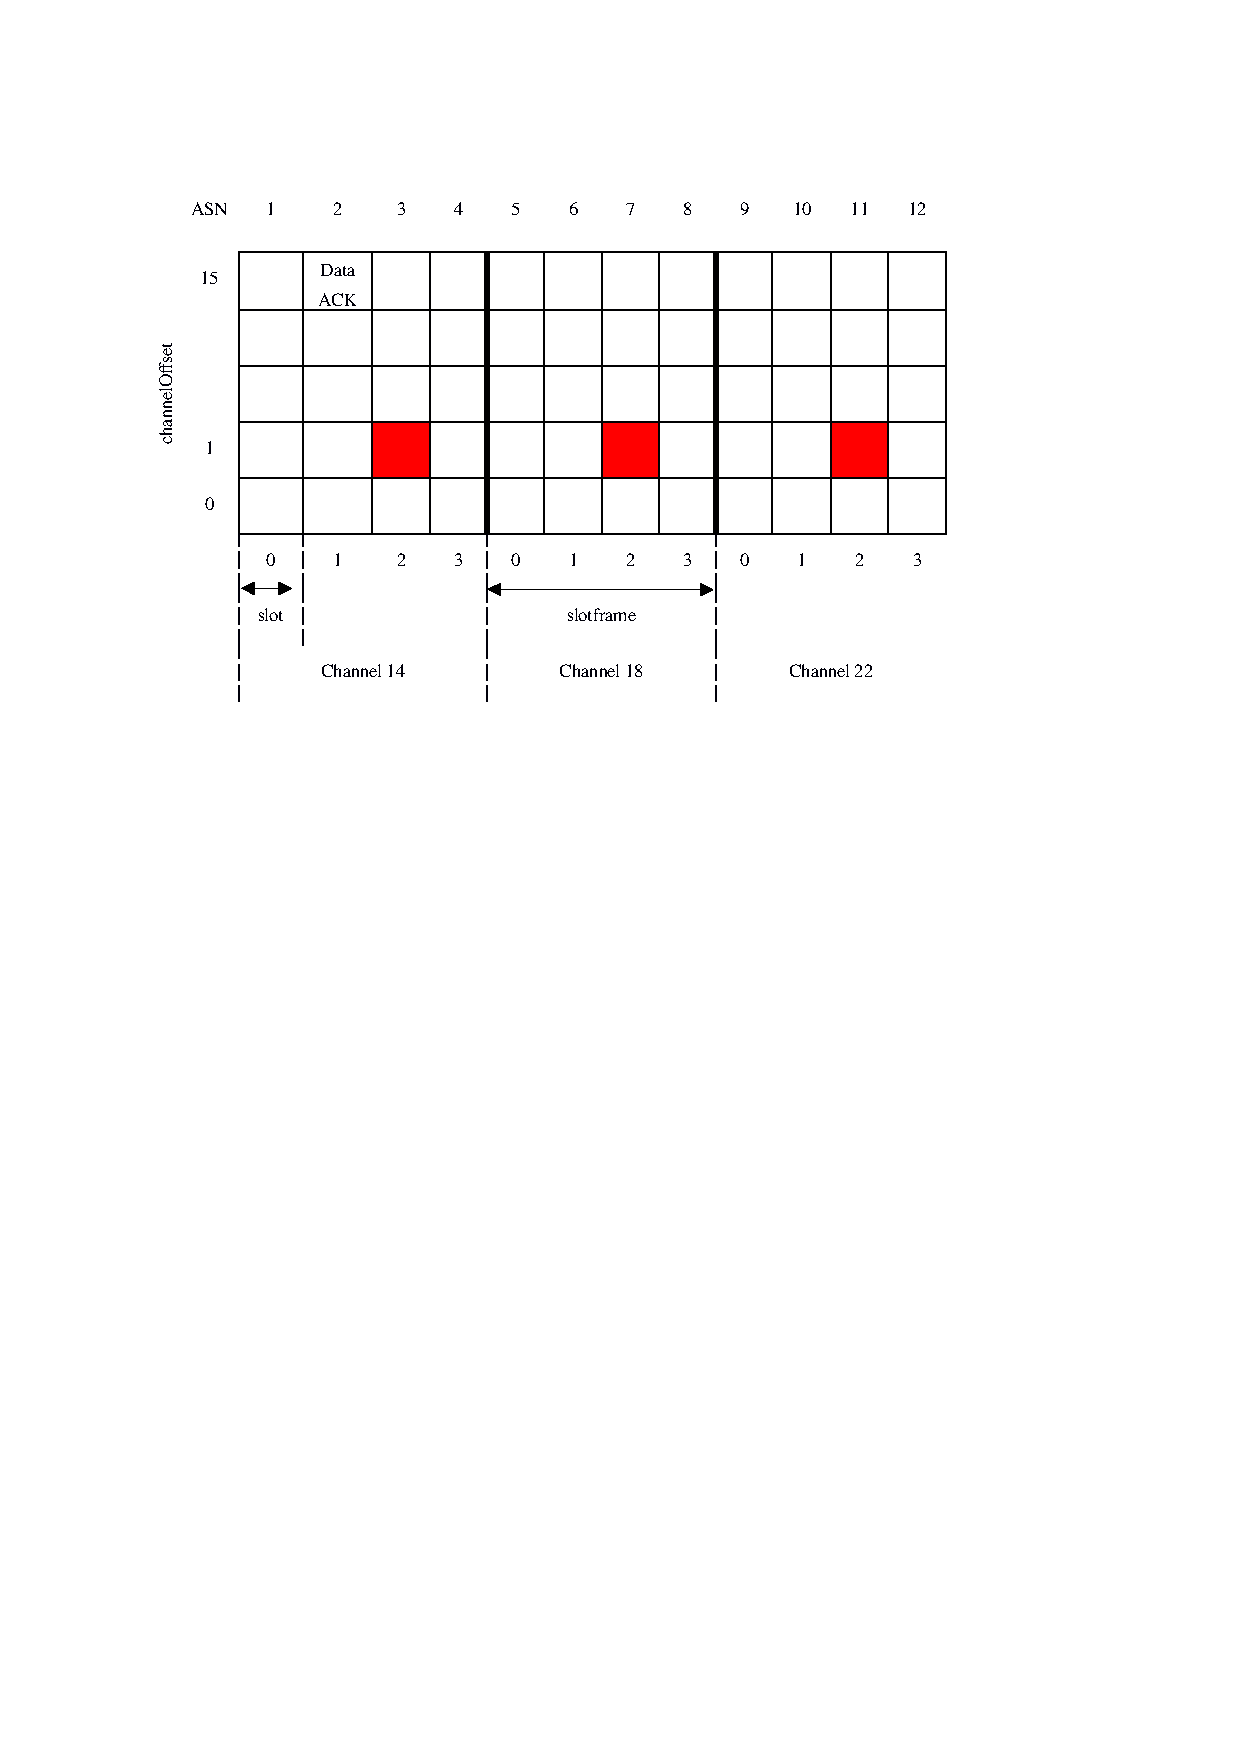
\includegraphics[trim=2cm 17cm 4cm 3cm, clip=true, totalheight=0.40\textheight]{tsch.pdf}
\caption{TSCH schedule}
\label{fig_tsch}
\end{figure}

\textit{Slotframes} contain a group of time slots of equal length and priority where the slotframe repeats continuously over time. The size of the slotframe is not appointed by TSCH. Shorter slotframe has the advantage of more available bandwidth as the result of frequent repetition of the same time slot but at the cost of higher power consumption. 

A single element in the TSCH schedule is called as a \textit{cell}. The cell can instruct the node to transmit, receive or sleep. It can also be marked as both transmitting and receiving. However, transmission takes precedence over reception. The TSCH schedule also indicates the channel and address of the node for communication. The channel in TSCH is referred as \textit{channelOffset}, which is the row in the TSCH slotframe. In a transmit cell, the outgoing buffer is checked for a packet that matches the scheduled neighbour for that time slot. Similarly, in a receive cell, the node listens during the reserve cell for possible incoming packets. Each scheduled cell is dedicated for the node. However, a cell can be shared where multiple nodes can transmit on the same frequency at the same time. TSCH defines a backoff algorithm to avoid transmissions from nodes in the shared cells from congesting the network.

Absolute Slot Number (ASN) is a timeslot counter in TSCH that calculates the communication frequency for the sender and receiver nodes. The calculation from ASN and \textit{channelOffset} is translated into a different frequency at different slotframe cycles. The ASN value changes at the next iteration which results in a different frequency computed for the cycle. This results in \textit{channel hopping} where the pairs of neighbours hop between different channels at each iteration.

The advantage of channel hopping is to have retransmission on a different channel than it was transmitted previously. The new channel is likely to be a more stable link. Otherwise, it will hop to another channel on the next cycle. This increases the likelihood of succeeding than retransmitting on the same channel, thus, forming a more stable topology. Nodes on different channels are allowed to run simultaneously on the same time slot as it does not interfere with each other transmissions. Channel hopping technique helps to combat external interference and impact the nodes differently on the channel.

%%Use 5 channels in the experiment.) The sequence number generation algorithm must guarantee that there is only one node among one-hop neighbors on any particular channel. The receiving node transmits a smal 

%%%How the schedule is built, updated and maintained is outside of the scope of the IEEE 802.15.4e standard. 

%%Nodes already part of the network can periodically send EB (Enhanced Beacons - contains timing information,In general, TDMA-based MAC protocols allocate a time slot to each node in the network. The allocated time slot is used for data transmission or data reception according to the protocol. channel hopping information, timeslot and slotframe information) frames. EB frames are sent on all  frequencies. A node wishing to join the network listens for EBs. The joining node can listen on any frequency until it hears an EB. What frequency it listens on is implementation specific. The new node enables the TSCH mode and use the information from the EB to synchronize to the network and it knows how to contact other nodes in network. \cite{tsch}

\subsubsection{MC-LMAC}
Multi-Channel Lightweight Medium Access Control (MC-LMAC) is a fully distributed schedule-based multi channel MAC protocol that is based on a single channel LMAC \cite{lmac}. The nodes periodically use a timeslot to schedule the transmission to avoid contention. MC-LMAC does not require a centralised scheduler for timeslot allocations; instead, it is done locally by the nodes by exchanging information of their slots and channels with the local neighbours. 

In MC-LMAC, the timeslots are selected with channels. The node can use the same timeslot used by a two hop neighbour if it is on a different frequency. However the node cannot use the timeslots on any frequencies that is used by the neighbours. The timeslot is selected autonomously. The node uses the same timeslot in the next frames if it does not conflict with the other nodes transmission in that slot. Otherwise, a new time slot is selected. The timeslot list is called \textit{occupied slot vector} where it stores the information about the neighbours' occupied slots. The slot vector is per channel where the node can selects a timeslot for each channel given that the timeslot is free.
The occupied slot vector is transmitted during the node's timeslot to the potential transmitters. All nodes are given the opportunity to select an empty slot for transmission.

\begin{figure}
\centering
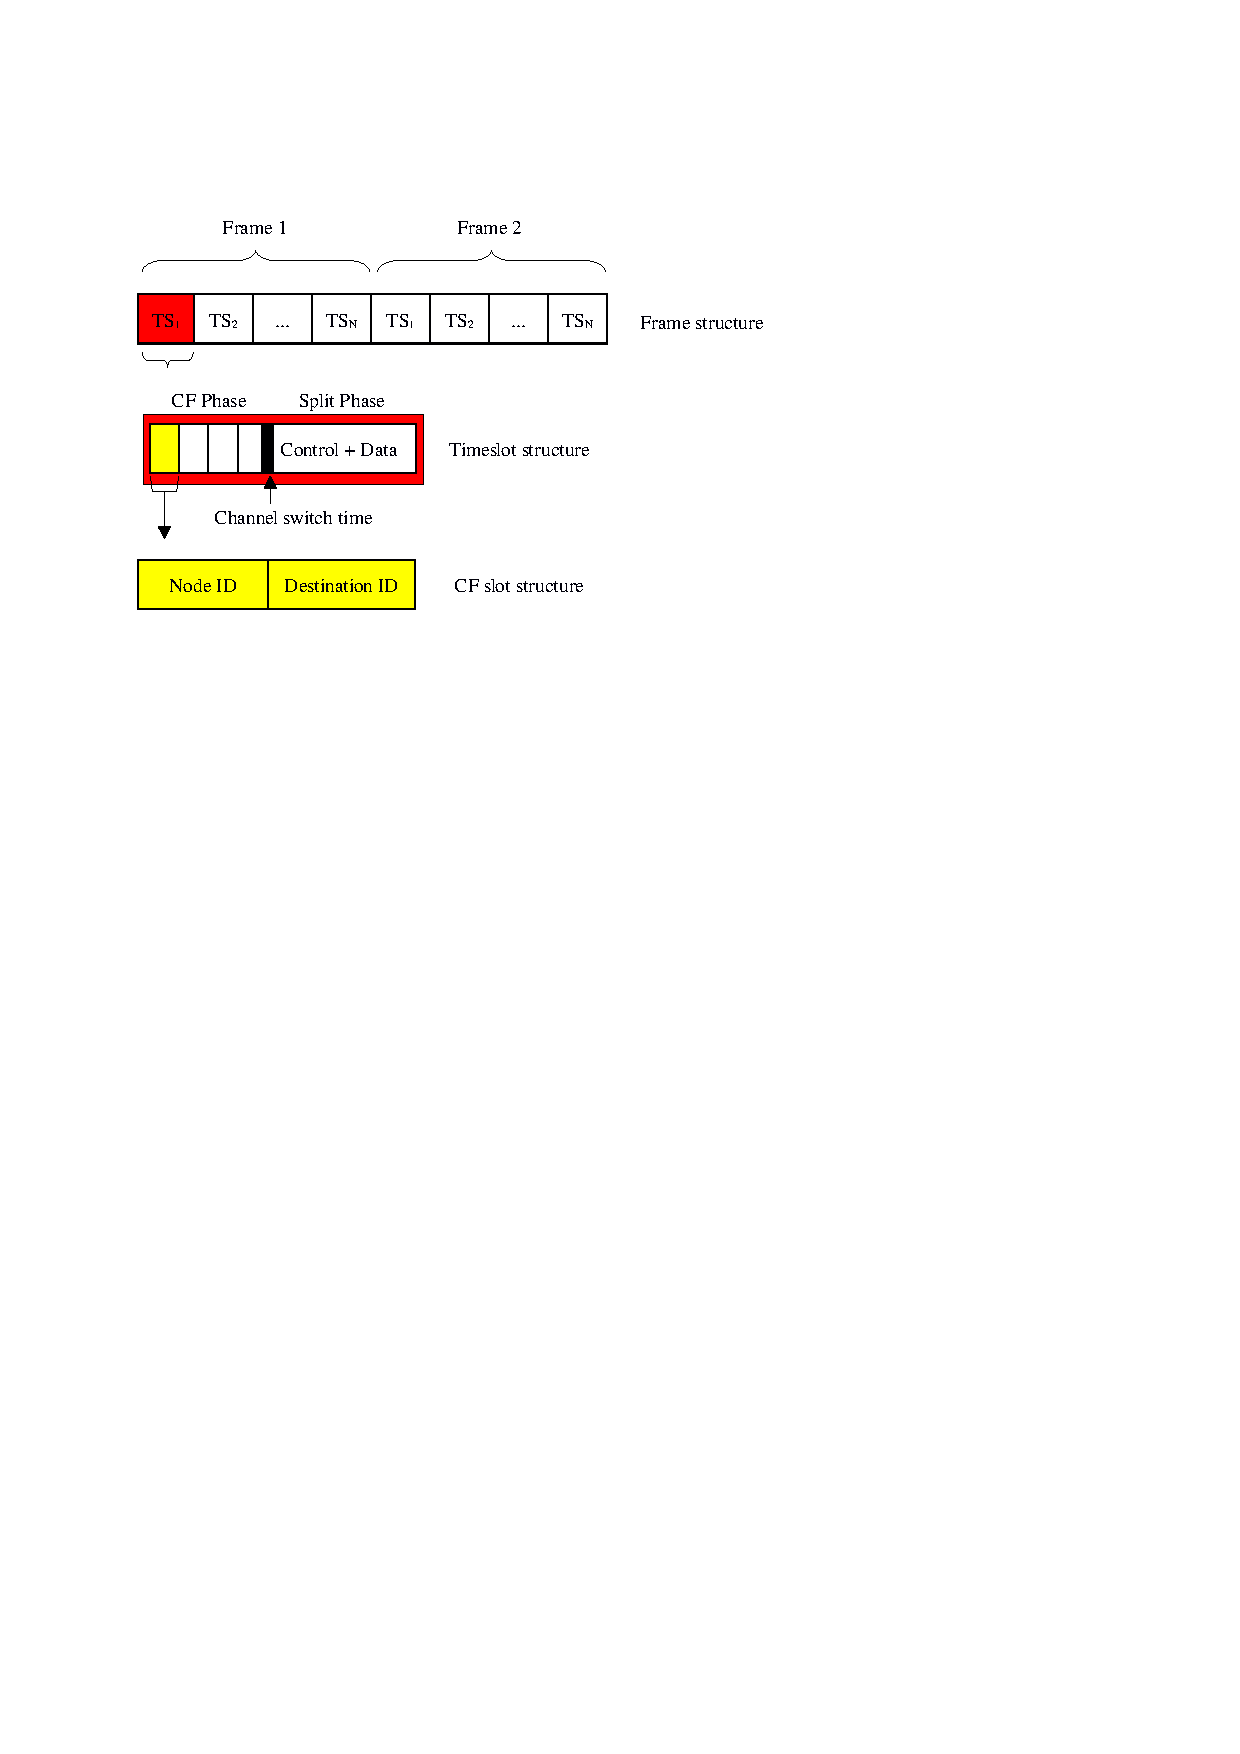
\includegraphics[trim=2cm 19cm 8cm 3cm, clip=true, totalheight=0.35\textheight]{mclmac.pdf}
\caption{MC-LMAC scheduling}
\label{fig_mclmac}
\end{figure}

A timeslot consists of a \textit{common frequency phase} (CF) and a \textit{split phase} as shown in Figure \ref{fig_mclmac}. All nodes listen on the common channel at the beginning of each timeslot in the CF phase to exchange control information with the neighbours. The common channel can be used for data transmission. The control information consists of the node's id and the intended destination id. The receivers listen during the whole CF phase. If it is the intended destination, the node switches to the sender's channel, otherwise it goes into the passive state. MC-LMAC uses the CF slot number as the senders channel number to avoid sending an extra transmission to the destination node.

Nodes can send broadcast messages by transmitting a broadcast address during the CF slot where the receivers switch to the sender's channel. A dedicated broadcast channel is not required. However, the CF duration increases when more channels are used which resulted in longer listening period thus energy to wait for potential incoming packets.

The senders and the intended receivers switch to the channel where the control message and data transmission will take place in the split phase. The sender sends a control message in the form of preamble packets before proceeding with transmitting the data message. The control message that is transmitted in the split phase includes the occupied slots list. The node also sends the current slot and slot numbers in the control message prior to data transmission to detect synchronisation error by compare the slot and frame numbers that it receives in the control message with its slot and slot number. In MC-LMAC, the synchronisation is done by synchronising nodes near to the sink with the sinks and continues hop by hop where the nodes synchronise with the parents. 
 
%!To select a free time slot, the potential receivers transmit a list of the timeslots during its timeslot that they are receiving. %The node selects its time slots from the list that is free. 

%!All nodes switch to the common control channel at the beginning of each timeslot in the CF phase to address their destination and to be informed whether they are addressed in the current slot. 
%!The intended destination id and node id are transmitted during the CF phase to notify the destination node to switch to the sender's channel. 

%!A common channel is used during CF period of each timeslot to inform receivers of the requests and channels of the transmission data and to collect information about the neighbours. 
%!The sender's channel number is the index or CF slot number that the destination node receives to avoid (reduce) extra transmission. 

%%Present a multi-channel MAC protocol, MC-LMAC, designed with the objective of maximizing the throughput of WSNs by coordinating transmissions over multiple frequency channels. MC-LMAC takes advantage of interference and contention-free parallel transmissions on different channels. It is based on scheduled access and dynamically switches their interfaces between channels. Time is slotted and each node is assigned the control over a time slot to transmit on a particular channel. 

%%Multi-Channel Lightweight Medium Access Control (MC-LMAC) is a schedule-based multi-channel MAC protocol that takes advantage of contention and collision-free parallel transmissions on different channels. 

\subsubsection{YMAC}
Y-MAC \cite{y-mac} proposed a multi channel MAC protocol that uses a light weight channel hopping mechanism. In Y-MAC, time is divided into several fixed-length frames. Each frame consists of a broadcast and unicast period. The broadcast traffic is separated from the unicast traffic for a more reliable broadcast where they do not share the same queue. Figure \ref{fig_ymac} shows the Y-MAC scheduling. At the start of the broadcast period, all nodes must wake up to exchange broadcast messages. The nodes switch to the base channel to transmit or receive the broadcast message. Broadcast messages are only exchanged during the broadcast period. The nodes turn the radio off if there is no incoming broadcast message. The nodes will wake up again during the unicast traffic time slot. Y-MAC exploits multi channel for unicast to reduce the packet delivery latency while using a single channel which is the base channel for broadcast messages.

\begin{figure}
\centering
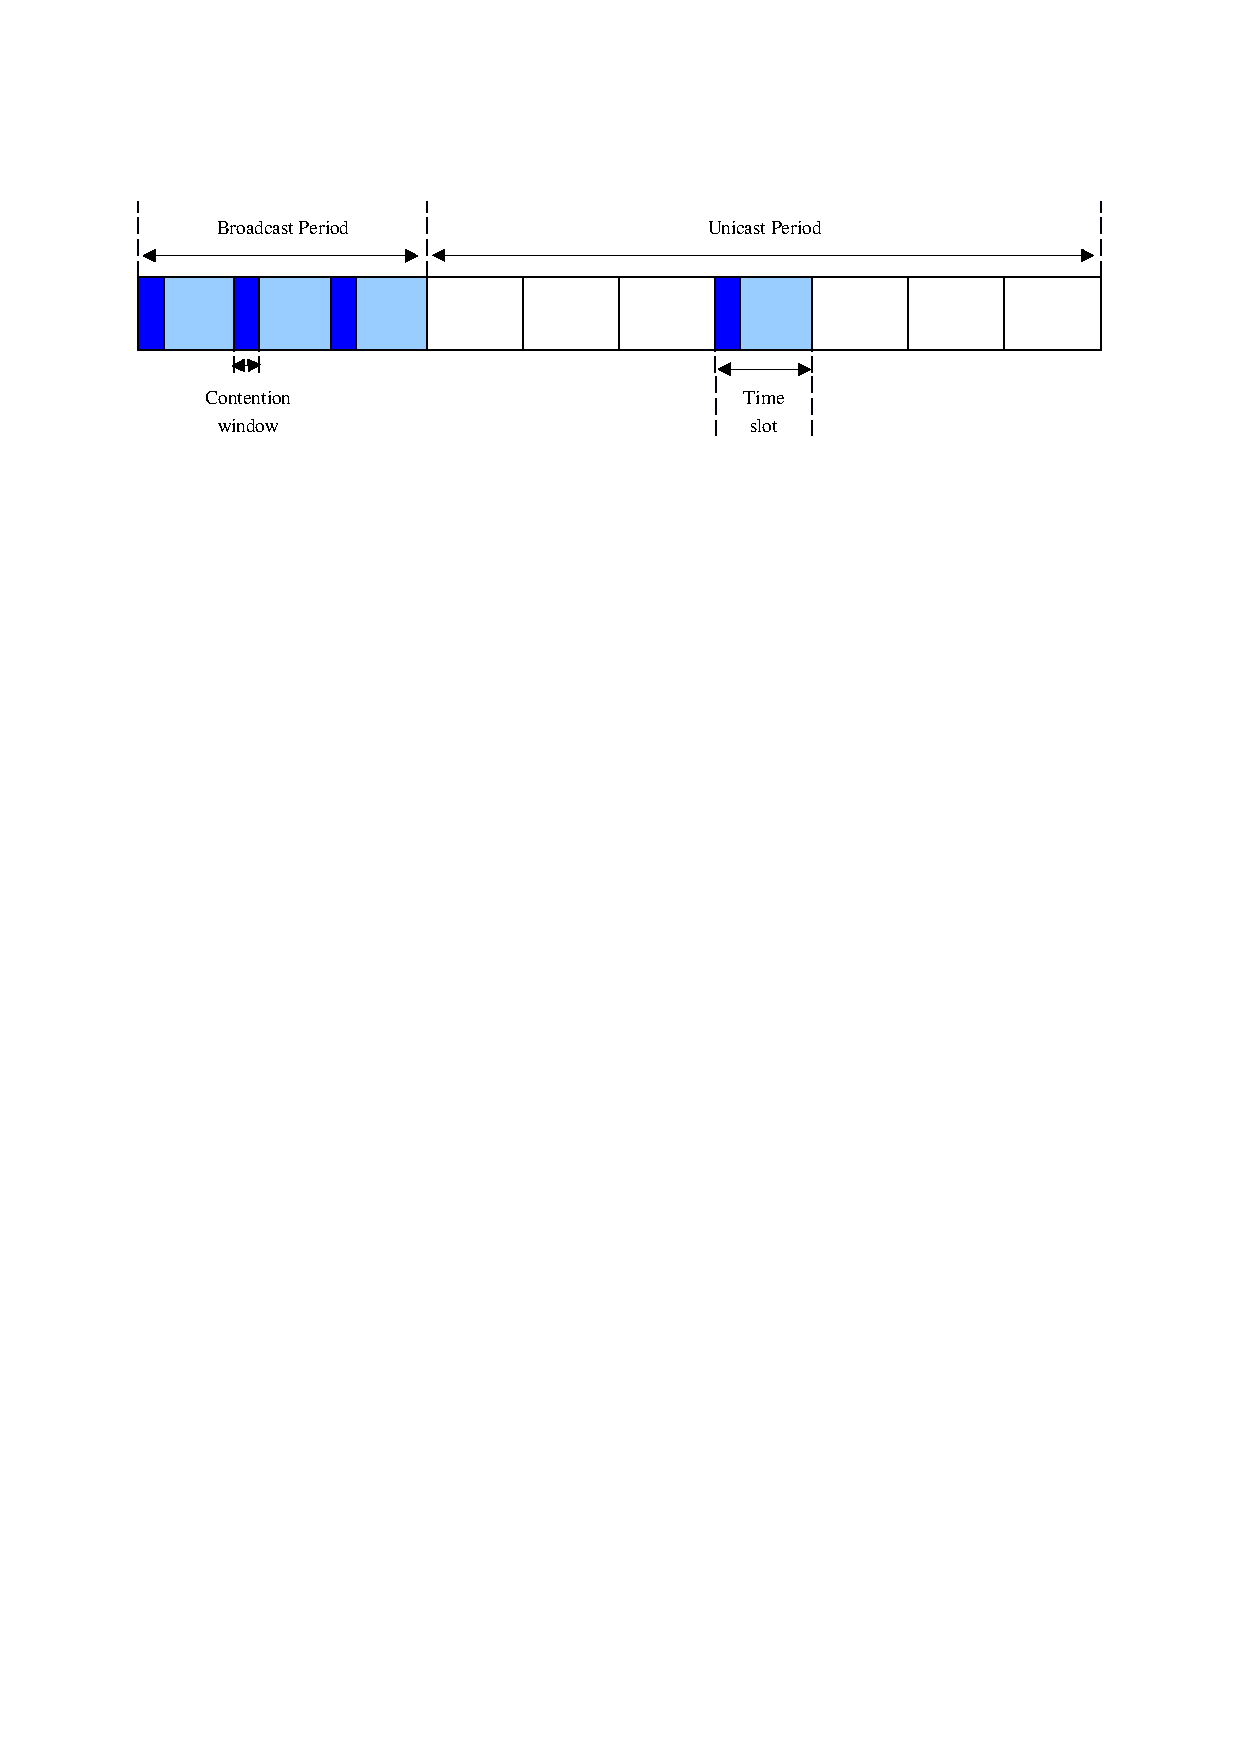
\includegraphics[trim=2cm 22cm 2cm 3cm, clip=true, totalheight=0.17\textheight]{ymac.pdf}
\caption{Y-MAC scheduling}
\label{fig_ymac}
\end{figure}

Y-MAC is a receiver based scheduling where the node checks the channel for incoming packet in its receive time slot. The time slot length is defined to be long enough to receive one message. The potential senders have to compete to be able to transmit. However, only the contention winner can transmit the packet to the receiver. The sender node sends a preamble until the end of the contention window if the channel is clear to withhold competing transmissions. At the end of the contention window, the receiver wakes up to receive the data. The receiver node transmit a small and independent packet at the start of the time slot to notify the potential senders if it waits in the next time slot for the senders to retry.

The receiver initially starts the hopping sequence on the base channel to receive the data. The receiver and potential senders hop to another available channel according to the hopping sequence to receive the following packet. The potential senders that have pending messages for the receiver will hop to the next channel and compete to transmit. The burst of messages ripple across channels which means that only one node uses the base channel at a time. This guarantees that each node will receive a packet on the base channel before it hops to another channel. The hopping sequence ensures that for any particular channel, there is only one node among one hop neighbour.

In Y-MAC, the nodes exchange the time remaining to the start of the next frame period. This information is included in the control message that is sent periodically as a broadcast to minimise the control overhead for time synchronisation. The receiving node that receives the time synchronisation information adjusts the expiration time of its timer by averaging the time remaining to compensate any timing error so that the start time to the next frame period is shorter. Time synchronisation is an important aspect in ensuring the network connectivity for communications.

%%A sender and a receiver have to agree on the communication channel as well as the transmission timing. This necessitates time synchronization algorithms. In Y-MAC, sensor nodes synchronize their upcoming timer events by exchanging the time remaining in the current superframe period. 
 
%%Sink periodically broadcasts control messages to initiate the network. A node which is trying to join the network turns on its radio transceiver to receive this timing information. Once a node receives the first control message, it sets its time remaining to the next frame period to equal that of the sender.

%%Y-MAC avoids redundant channel assignment by not allocating fixed channels to the nodes. 

%%There's a tradeoff between the number of time slots and the delivery latency. The more time slots we have, the more nodes we can allocate exclusive time slots to, but delivery latency increases due to the prolonged length of the frame period. 

\subsection{Asynchronous Systems}
%-EM-MAC, MuChMAC, Chrysso, MiCMAC - ContikiMAC?
Recent asynchronous multi channel MAC protocols are Chrysso and MiCMAC. These protocols are using Contiki operating system. MiCMAC is built based on ContikiMAC, the default radio duty cycling in Contiki 2.7 that works in a single channel. The details of these are explained below. The single channel ContikiMAC is also explained as the duty cycling mechanism in ContikiMAC is important in MCRP, the protocol proposed in this thesis.

\subsubsection{ContikiMAC}
ContikiMAC \cite{contikimac} is the default radio duty cycling mechanism in Contiki 2.7. It is an asynchronous system where it does not need scheduling, signalling messages, and additional packet headers. It uses periodical wake ups to listen to incoming packets from the neighbours. Periodical wake ups has been used by many protocols such as B-MAC \cite{bmac}, X-MAC \cite{xmac} and BoX-MAC \cite{boxmac}. 
ContikiMAC default wake up frequency is set to 8 Hz which results in a wake up interval of 125 ms. Frequent wake up would enable quicker packet detection in the case of frequent packet transmissions at the cost of higher network power consumption.

The receiver is kept on when it detects a packet transmission during a wake up. ContikiMAC wake ups use an inexpensive \textit{Clear Channel Assessment} (CCA) that relies on the threshold of the \textit{Received Signal Strength Indicator} (RSSI) to signify the radio activity on the channel. A positive CCA represent a clear channel if the RSSI is below a threshold and the CCA returns a negative value if the channel is currently in use. The ContikiMAC CCAs do not detect packet transmission. They are used to detect the activities on the radio signal which could be that (i) a neighbour is transmitting to a receiver, (ii) a neighbour is transmitting to other receivers, or (iii) other devices that radiate radio energy. 

ContikiMAC uses a fast sleep optimisation to enable the receivers to quickly go to sleep in the case of spurious radio interference that is a false positive wake ups. The receivers can go back to sleep if (i) the duration of the radio activity is longer than the maximum packet length, (ii) the silence period is longer than the interval between two successive transmissions or (iii) the start of packet is not detected.

Another feature of ContikiMAC is the transmission phase-lock mechanism. This feature has been suggested by WiseMAC \cite{wisemac} previously and has been used by other protocols. In Contiki, the phase-lock optimisation is implemented as a separate module from ContikiMAC. It manages a list of neighbours and their wake up phases. 

\begin{figure}
\centering
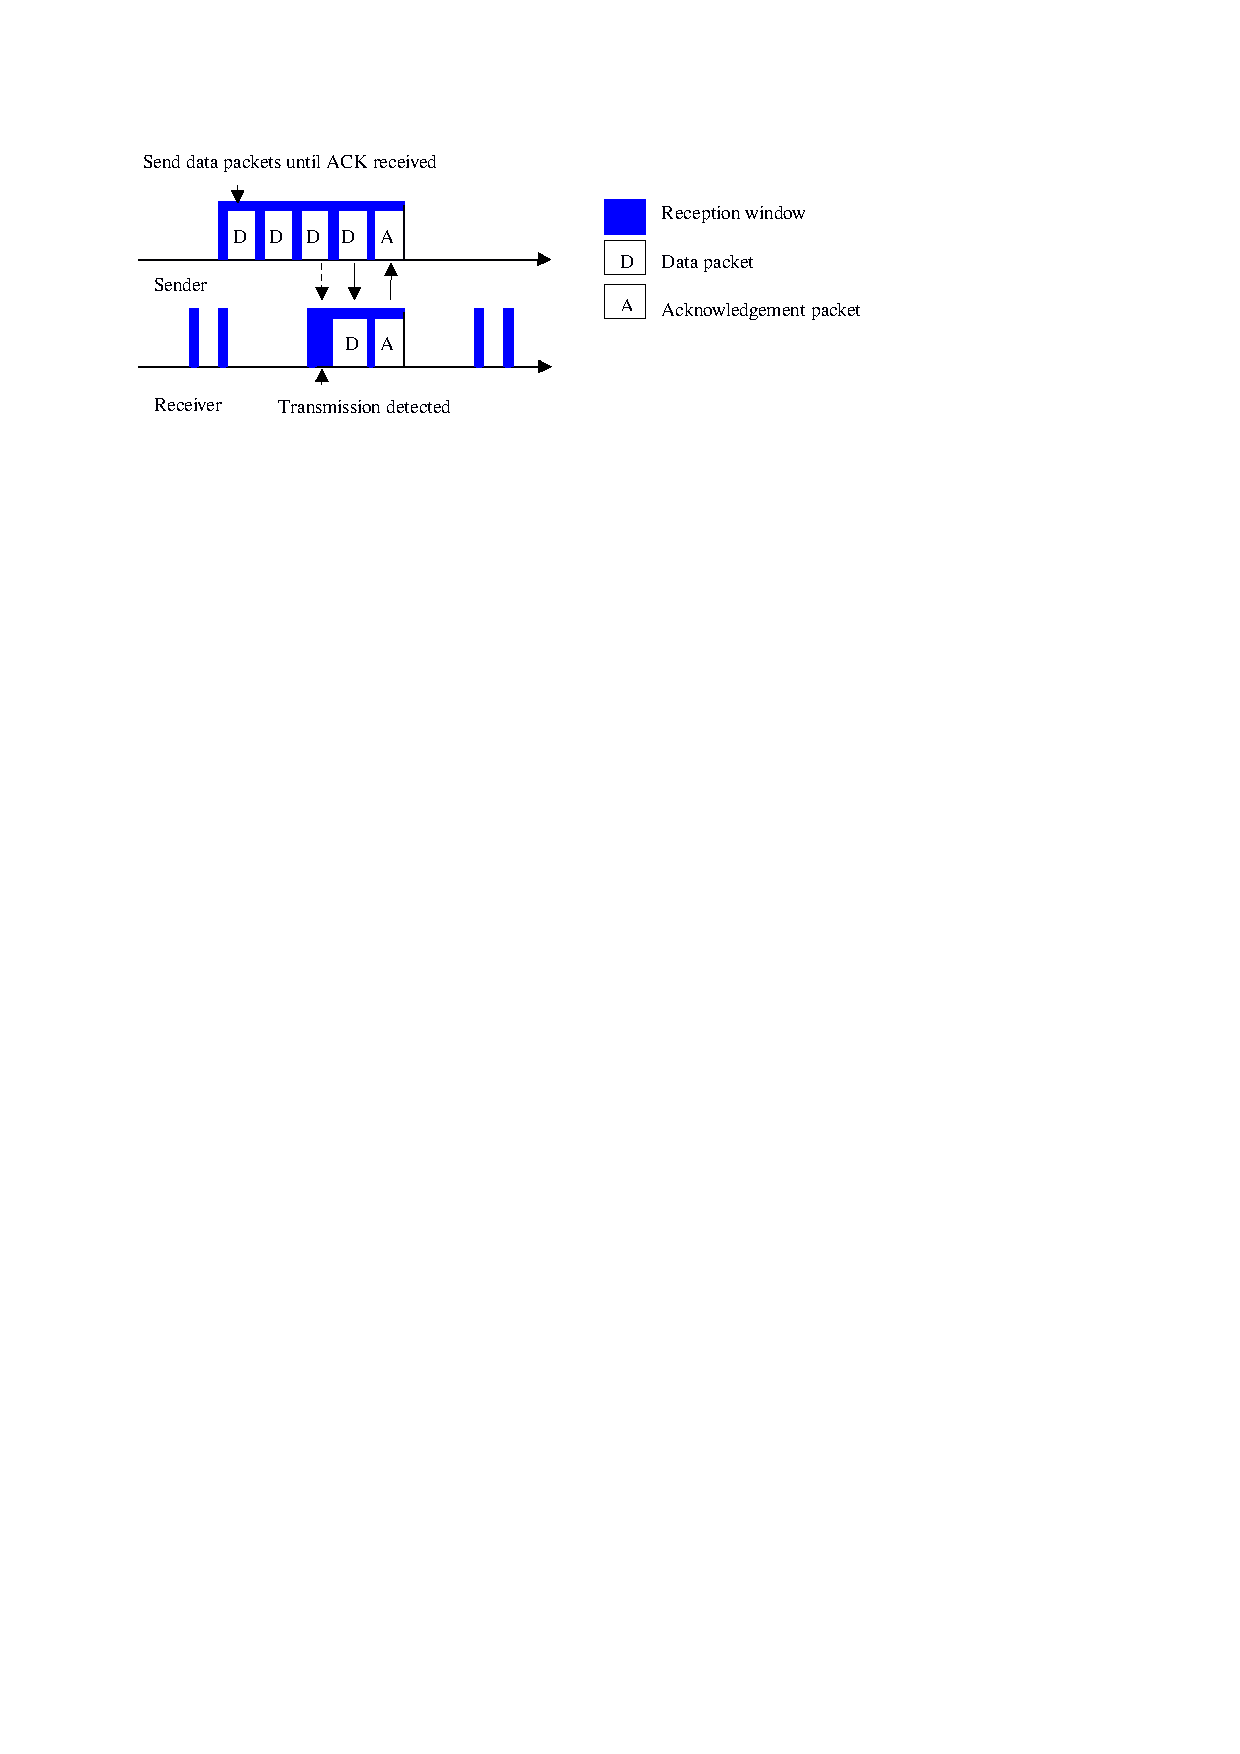
\includegraphics[trim=2cm 22cm 6cm 2cm, clip=true, totalheight=0.25\textheight]{contikimac.pdf}
\caption{ContikiMAC unicast transmission}
\label{fig_contikimac}
\end{figure}

When a sender has a packet to send, the sender repeatedly sends the packet until it receives a link layer acknowledgement from the receiver to indicate that the packet has been successfully received. Figure \ref{fig_contikimac} shows ContikiMAC unicast transmission. A sender can learn the receiver's wake up phase through the link layer acknowledgement. This reduces the number of transmissions required significantly as the sender can send the packet shortly before the receiver is expected to be awake which as a result, reduces the network congestion.

However, a broadcast packet does not result in a link layer acknowledgement. The packet is instead repeatedly sent in the full wake up interval to reach all neighbours. During broadcast, the sender can turn the radio off between each packet transmission to save power as it does not expect to receive any link layer acknowledgement.

%%a transmission phase-lock optimization, to allow run-time optimization of the energy-efficiency of transmissions. 

%%%ContikiMAC must be able to discern between these events and react properly.

\subsubsection{MiCMAC}
MiCMAC \cite{micmac} is a distributed channel hopping variant of ContikiMAC. It inherits ContikiMAC basic design and further extended to support multi channels. It also extends ContikiMAC's phase lock to include \textit{channel lock} for wake up channel. MiCMAC is independent from the other layers in the protocol stack. It is compatible to run with RPL routing.

In MiCMAC, the node switches to different channel each time it wakes up. The channel is generated using a Linear Congruential Generator (LCG) for a pseudo-random sequence. The generated sequences are random and use each possible number within the range once before the sequence is repeated. MiCMAC uses a predefined hopping sequence that is provided in a static table of all sequences instead of generating the hopping sequences at runtime to increase optimisation. The sequence is selected according to the node's MAC address.

When communication with the neighbour for the first time, the sender transmits strobes repeatedly on a channel for a maximum number of channels wake up. The sender picks any channel. The receiver wakes up on different channel each time following the pseudo-random sequence and it will wake up exactly once on the sender's strobing channel. The receiver sends an ACK that includes the node's pseudo-random generator parameters. The sender will use this information and the number of periods elapsed since the last successful unicast with the receiver to generate the next wake up channels for the node.

The sender switches to the receiver's expected channel just before it wakes up, checks the radio activity using CCA and sends the packet if the channel is clear. The receiver will reply with an ACK to the sender. The sender updates its information of the receiver's wake up time and channel before it goes back to sleep. If the ACK is not received, the sender assumes that the receiver's wake up time and channel is wrong. The sender updates the receiver's information. 

\begin{figure}
\centering
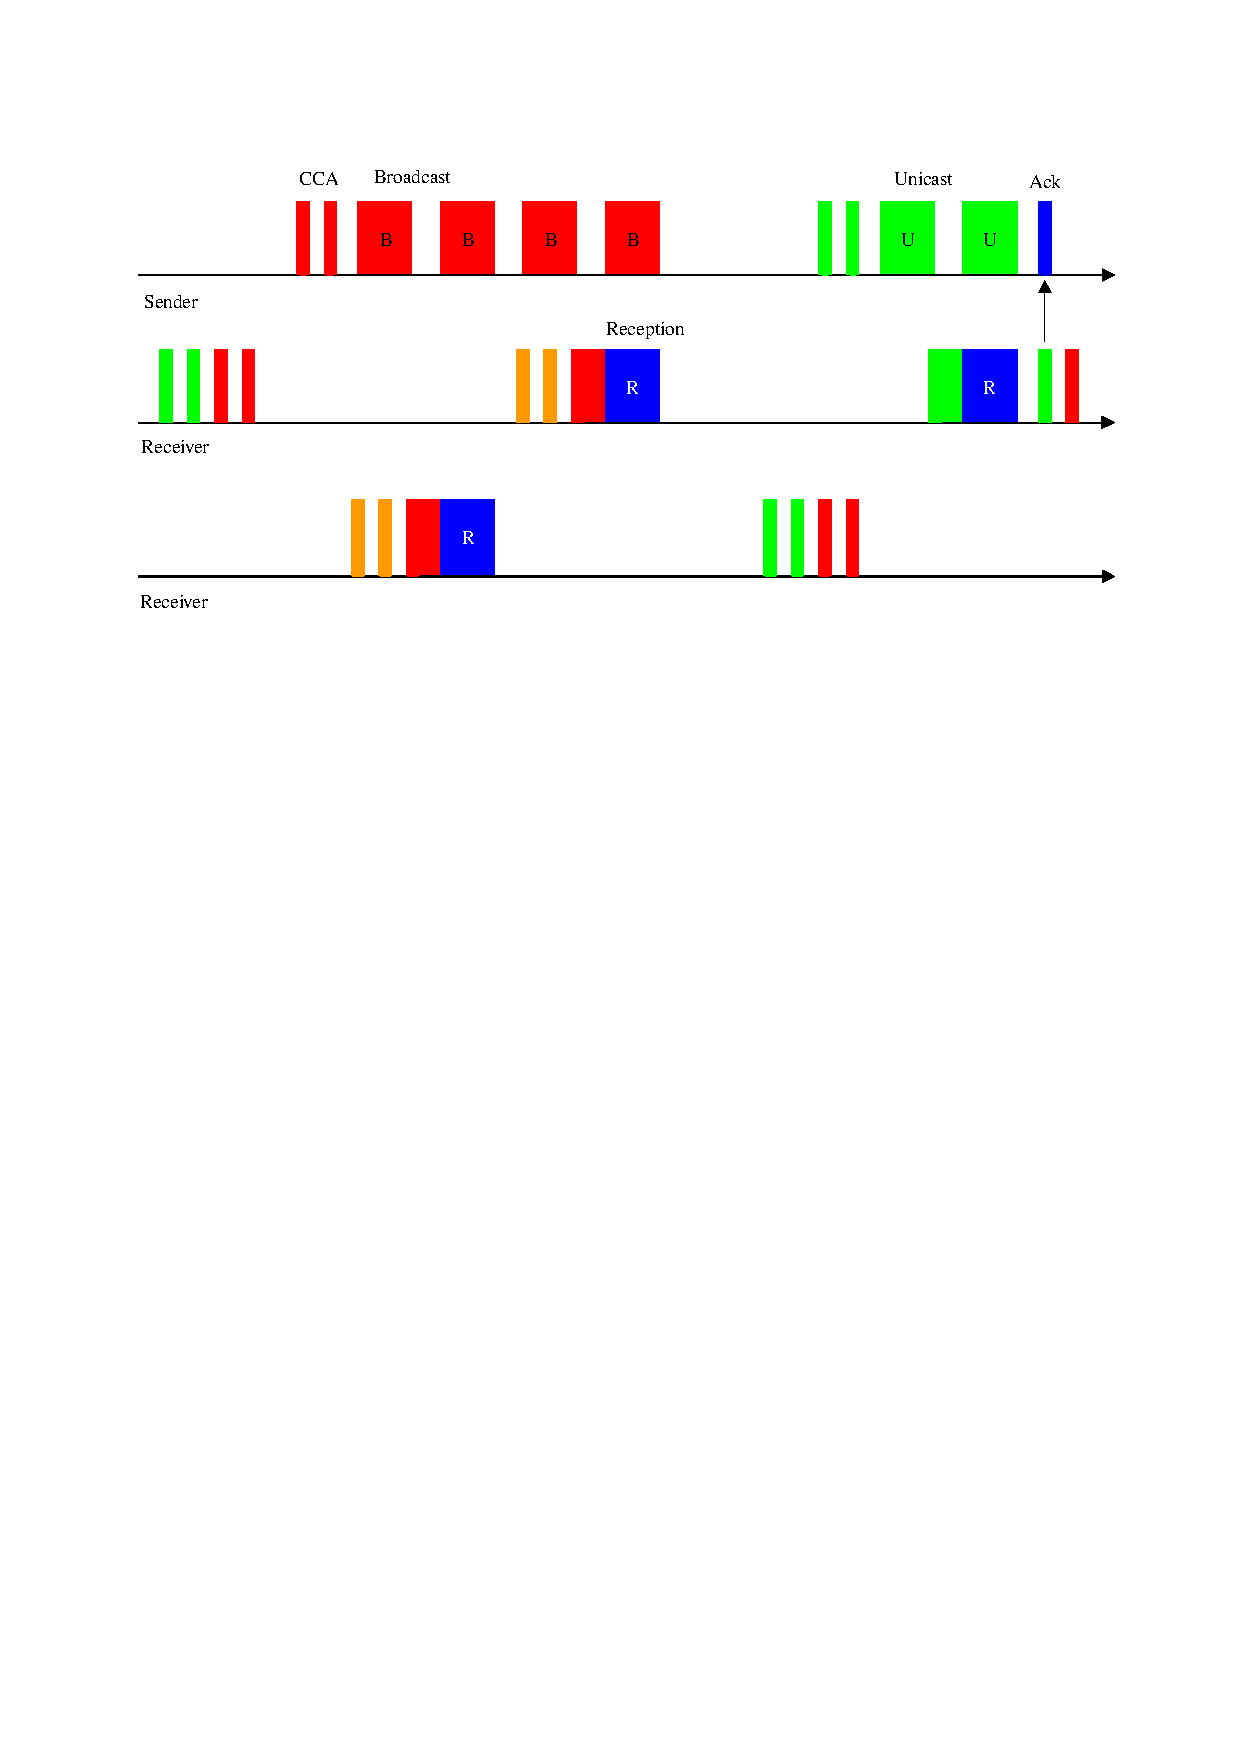
\includegraphics[trim=2cm 19cm 1cm 2cm, clip=true, totalheight=0.30\textheight]{micmac.pdf}
\caption{MiCMAC unicast and MiCMAC-BC transmissions}
\label{fig_micmac}
\end{figure}

MiCMAC supports broadcast and introduces two variants of MiCMAC; MiCMAC and MiCMAC-BC. In the basic MiCMAC broadcast, only one of the available channels in the sequence is strobes continuously for a maximum number of channels wake up. It has the disadvantage of increased energy and channel used from the broadcast message. MiCMAC-BC on the other hand uses a dedicated broadcast channel. The nodes wake up on the broadcast channel at every period in addition to the unicast pseudo-random wake up channel. However, it has the disadvantage of reduced robustness as the broadcast channel is fixed and MiCMAC requires two wake ups at every period which are for the broadcast, followed by the unicast channels. Figure \ref{fig_micmac} shows MiCMAC-BC and unicast transmissions.

In MiCMAC, the performance degraded when it considers all 16 channels as it includes the high interference channels for transmissions. It also increases the broadcast and channel-lock costs. MiCMAC showed an optimal performance with 4 channels. 

%%The per-channel measurements are not strictly required for MiCMAC to operate but do them for the sake of fair comparison. Channel diversity which increases the number of usable links due to different signal propagation obtained when hopping to a new channel. Channel diversity also leads to a more stable topology, reduced number of parent switches. MiCMAC hides losses from the routing layer, resulting in a more stable topology. \cite{micmac}

%%Advantage when we want to find a node's wakeup channel. Do blind channel hopping because of simplicity as local blacklisting would involve some overhead for synchronizing the blacklists among neighbours. "Previous work has shown that even random blind channel hopping improves network connectivity, efficiency and stability when compared to single-channel"///reference??//. 

\subsubsection{Chrysso}
Chrysso \cite{chrysso} is a multi channel protocol extension that is specifically tailored for data collection applications. Chrysso is implemented in Contiki 2.4 using \textit{collect} routing protocol which is a data collection. Chrysso switches the channel of the nodes that are affected by the external interference to a new set of channels when the interference is detected to evade the interference source.

Chrysso allows the parent to coordinate the channel switch when interference is detected for each individual parent-children group. Chrysso operates on two channels; one for incoming (called as inchannel) and the other channel is for outgoing (outchannel) traffic. Chrysso maintains a pre-defined logical list of available channel. The parent and children use this list to ensure consistency when they are switching to the next channel. Chrysso implemented five channels which are channel 26, 14, 20, 11 and 22 and evaluated Chrysso's performance using these channels in this particular order.

Chrysso consists of a set of control loops; the inner and outer loops, that decides to maintain or switch the parent-children's channel. The inner loop is responsible for the parent-children channel switching coordination when there is external interference. The child node collects data from the channel quality monitor periodically which is then included onto the data packet. The parent uses the average over congestion backoffs values to measure and determine if there is external interference in the current measured channel quality. If the computed value exceeds a predetermined threshold, the children are notified of the channel switching request before the parent switches to the next inchannel.

Chrysso uses the outer loop during severe interference that blocks any communication where the parent-children channel switching coordination could not be invoked. The outer loop is a watchdog mechanism where autonomous channel switching is initiated when the inner loop could not be triggered. The nodes, both parent and children independently switch to the next channel in outer loop. The child node monitors the number of failed transmissions. If it exceeds a predefined threshold, the outchannel is switches as it indicates that the channel has severe interference. Likewise, the parent records the number of packets it received and switches to the next inchannel instantly and autonomously if the received packets are below a pre-set threshold value of the expected packets.

The watchdog initiates the \textit{scan mode} to find a new parent when the nodes have lost contact with the parent after the channel switches. The node scans through all available channels except the previously used outchannel to find a new parent as neighbours are now operating on different channels. The scan mode is triggered on demand as it uses additional overhead for processing and consumes energy. 

%%***Fundamental problem of multi-channel protocols: channel deafness (not hearing a packet on a different channel). \cite{chrysso}

%%//inner, outer, scan
%%Chrysso is a multi-channel protocol extension, that leverages the channel diversity of sensor node radio.  

\subsection{Comparison and Discussion}
The reviewed MAC protocols features are summarised in Table \ref{table:macProtocol}. Several issues that exist are in term of:

\begin{table}
\centering
\begin{tabular}{|C{2cm}|C{2cm}|C{2.4cm}|C{2cm}|C{2cm}|C{1.8cm}|}
\hline
Protocol & Medium Access & Channel Assignment & Channel Switching & Common Period & Broadcast \\
\hline \hline
TSCH & TDMA + collision window & Dynamic & Once per cycle & No & Yes \\
MC-LMAC & TDMA & Senders & Once per time slot & Yes & Yes \\
Y-MAC & TDMA + collision window & Dynamic & Once per time slot & Yes & Yes \\
MiCMAC & MiCMAC & Dynamic & One per wake up time & Yes & Yes\\
Chrysso & ContikiMAC & Dynamic & When require & No & No\\
\hline 
\end{tabular}
\caption{Comparison of studied MAC protocols}
\label{table:macProtocol}
\end{table}

\begin{enumerate}
\item \textbf{Synchronous versus asynchronous design} - 
Both designs have their advantages and disadvantages. However, synchronous MAC protocols require the network topology to be known before it can schedule timeslots to avoid conflict between the nodes. Asynchronous MAC protocols depend on the channel condition and the nodes compete for the channel access.

\item \textbf{Sender versus receiver initiated design} - 
Most MAC protocols presented are both sender and receiver initiated where the channel decisions depended on both nodes.

\item \textbf{Channel hopping design} - 
The channel quality checking at run time costs a lot of energy. In most of the MAC protocols studied evaluation, the protocols are tested using a few selected channels instead of considering all available channels. This limits the spectrum usage of the frequencies.

\item \textbf{Broadcast support} - 
Most MAC protocols presented provide a broadcast support except for Chrysso. The protocols specified a broadcast period at every wake up on a fixed channel which reduces the robustness of the protocol as broadcast will occurs on the same channel each time. TSCH on the other hand treats broadcast message the same as a unicast message where it needs to select a slot before it can proceed but with a broadcast MAC address as the destination.
\end{enumerate}

Based on these reviews, the MAC protocols have many features that ease the multi channel processes. However, to further improve multi channel protocols, cross layers decisions are required. This could lighten the processing load at the MAC protocol and to allow switching decisions to be determined at run time on the upper layer which could compute better decisions.

\section{Routing Protocol}
\label{routingProtocols}
Routing protocols are responsible in routing data from the sender to the intended receiver across the network. In WSNs, the sensor nodes are restricted to a transmission range of approximately 20-30 metres indoors and 75-100 metres outdoor \cite{telosb-datasheet}. The routing protocols are required to manage and maintain the routes to ensure reliable communications between the limited range nodes. The routing protocols in WSNs are different than the traditional routing protocols as sensor nodes have limited processing capabilities, limited storage and use different operating system.

\subsection{Introduction}
In WSNs, flooding and gossiping are two classical approaches to relay data to the destination \cite{akkaya2005survey}. Gossiping is a slightly enhanced version of flooding. These data delivery approaches does not depend on any routing protocols and network topology. In flooding, the packet is broadcasts to all the node's neighbours and the neighbours that receive the packet will continue to broadcast the packet to their neighbours until the packet destination is found or the maximum number of hops allowed is reached. In gossiping, instead of flooding all the neighbours, it selects a random neighbour to forward the packet. The node that was selected will pick another random neighbour to continue sending the packet until it arrives at the intended receiver. Flooding and gossiping approaches are easy to implement. However, the approaches cause duplicated messages due to overlapping nodes that receive and send the same packet. The approaches also consume a large amount of energy. Gossiping causes propagation delay as the nodes selected are not guarantee to be the nearest node to get to the destination node.

Routing protocol is important in ensuring reliable packet delivery in WSNs. Several crucial criteria in the design of a routing protocol are in term of scalability, reliability, power consumption and adaptability. In WSNs, sensor nodes are typically densely deployed in the error prone wireless channels. This places the importance of scalability in the routing protocol to reduce conflict between the nodes and external interference from other devices while maintaining reachability between nodes. Sensor nodes are equipped with limited battery power. The routing protocol should consider the sensor nodes battery level before deciding on the routes. It can prolong the network lifetime by considering alternative routes in order to avoid draining lower energy nodes. Throughout the network lifetime, the nodes may fail, join or move to a different location than the nodes were initially. The routing protocol should be able to adapt to these changes and updates the routes accordingly.

Routing protocols are aimed to provides an optimised, scalable and energy efficient routes in the network which as a result, could prolong the network lifetime.

%%Reliability - must provide error control and correction mechanism to ensure reliable data delivery over noisy, error-prone and time-varying wireless channels.
%%Channel utilization - since sensor nodes have limited bandwidth resources, communication protocols designed for sensor network should efficiently make use of the bandwidth to improve channel utilization (MAC layer??).
%%Routing protocol approaches can be classified into () types which are flat based and data centric, hierarchical, location based and network flow and quality of service (QoA) aware.

\subsection{Classification of Routing Protocols}
There have been many routing protocols that were developed for WSNs. The routing protocols can be classified into 4 types \cite{akkaya2005survey}; (i) flat based and data centric, (ii) location based, (iii) network flow and quality of service (QoS) aware, and (iv) hierarchical based. These classifications are explained below with examples of the existing routing protocols for each type.

%%%There have been many routing protocols that were developed for WSNs. The routing protocols can be classified into 5 types \cite{akkaya2005survey}; (i) flat based and data centric where the protocols are query based and use meta data or data identification, (ii) location based where the node positions are used to reduce the area considered to relay the data, (iii) network flow and quality of service (QoS) aware where the QoS requirements are required to be fulfilled for routing, (iv) hierarchical based where the nodes are clustered and the data are aggregated at the cluster head to reduce the number or data and energy for the transmission, and (v) hybrid based where it combines several of the other techniques mentioned for a stable and energy efficient routing.

%%%The routing protocol is highly influenced by the data delivery model, especially in regard to the minimization of energy consumption and route stability. Similar to MAC protocols(????), the routing protocols can b for continuous, event-driven, query-driven and hybrid. In continuous delivery mode, each sensor sends data periodically. In event-driven and query-driven models, the transmission of data is triggered when an event occurs or a query is generated by the sink. Some networks apply a hybrid model using a combination of continuous, event-driven (sender) and query-driven (receiver) data delivery. \cite{akkaya2005survey}

\subsubsection{Flat based and Data Centric}
Data centric routing is a neighbour-to-neighbour query based routing. It uses attribute-based name or meta data to refer to a specific data. The sender sends data queries to a certain region and waits for the sensors to send a reply with the queried data. SPIN \cite{spin} and Directed Diffusion \cite{directeddiffusion} are a few examples of the earlier data centric protocols. 

SPIN is the first data centric protocol. It uses high-level descriptors or meta data to refer to the data. These meta data are exchanged using the data advertisement mechanism among sensors before transmission. Each node in SPIN is only required to know its immediate single hop neighbour. This allows topological changes to take place locally. The nodes that receive the meta data will then advertise the data availability it to its neighbours. This allows interested nodes to query the data.
%Disadvantage
However, SPIN does not guarantee the delivery of data to the interested node. The data delivery is decided by the nodes that are situated between the source and destination nodes. If the in between nodes are not interested in the data, the data will not be delivered to the destination.
%Advantage
%In SPIN, each node are only require to know it's immediate single hop neighbour. This allows topological changes to take place locally.

%%It negotiates data between nodes to eliminate data redundancy and reduce energy consumption during transmissions.


%In data-centric routing, the sink sends queries to certain regions and waits for data from the sensors located in the selected regions. Since data is being requested through queries, attribute-based naming is necessary to specify the properties of data. 

%%Data centric - all communication is neighbor-to-neighbor (no need addressing mechanism). 

%SPIN \cite{spin} is the first data-centric protocol, which considers data negotiation between nodes in order to eliminate redundant data and save energy.

Directed Diffusion is a query-driven data delivery model. It is an important milestone in data centric routing. Directed Diffusion aims at diffusing data using attribute-value schemes. The data on the sensor is queried in an on demand basis using the attribute-value pairs. An interest or task is defined using a list of attribute-value pairs to create a query. The sink broadcasts the interest through its neighbours. The interest is cached at the receiving nodes for later use. Caching helps to increase the routing energy efficiency and minimise delay. It is used to compare the received data with the values in the interests. The reply link to the neighbour from which the interest was received is called a gradient. The paths are established between the sink and sources based on the interest and gradient utilisation where one of the paths is selected as reinforcement. The interest is then resent by the sink using the selected path with a smaller interval. Directed Diffusion selects a new or alternative path that sends data in lower rates when the current path fails.

In Direction Diffusion, the sink queries the sensor nodes for the specific data. SPIN however, advertise the available data to allow interested nodes to query the data. There are many other protocols that have been proposed either based on Directed Diffusion such as Rumor Routing \cite{rumorrouting}, GBR \cite{schurgers2001energy}, CADR \cite{cadr}) or following a similar concept such as TEEN \cite{teen} which is also a hierarchical-based, and ACQUIRE \cite{acquire}.

%Difference: In Directed Diffusion, the sink queries the sensor nodes if a specific data is available by flooding some tasks. (sink to nodes)
%Advantages: Caching is a big advantage in term of energy efficiency and delay. Energy efficient since it is on demand and there is no need for maintaining global network topology.
%Disadvantages: Cannot be applied to all sensor network applications since it is based on a query-driven data delivery model.

%Later, Directed Diffusion \cite{directeddiffusion} has been developed and has become a breakthrough in data-centric routing. 

%SPIN - the idea behind SPIN is to name the data using high-level descriptors or meta-data. Before transmission, meta-data are exchanged among sensors via a data advertisement mechanism, which is the key feature of SPIN. Each node upon receiving new data advertises it to its neighbors and interested neighbors (sensors advertise the availability of data allowing interested nodes to query that data). 
%Difference: In SPIN, sensors advertise the availability of data allowing interested nodes to query that data. (sensor asks others if they want its data)
%Advantages: of SPIN is that topological changes are localized since each node needs to know only its single-hop neighbors. 
%Disadvantage: SPIN's data advertisement mechanism cannot guarantee the delivery of data. If the nodes that are interested in the data are far away from the source node and the nodes between the source and destination are not interested in that data, such data will not be delivered to the destination at all. 

%Directed Diffusion - is an important milestone in the data-centric routing research of sensor networks. The idea aims at diffusing data through sensor nodes by using naming scheme for the data. Direct Diffusion suggests the use of attribute-value pairs for the data and queries the sensors in an on demand basis by using those pairs. 
%The interest is broadcast by a sink through its neighbors. Each node receiving the interest can do caching for later use. The interests in the caches are then used to compare the received data with the values in the interests. A gradient is a reply link to a neighbor from which the interest was received. By utilizing interest and gradients, paths are established between sink and sources. Several paths can be established so that one of them is selected by reinforcement. The sink resends the original interest message through the selected path with a smaller interval. When a path between a source and the sink fails, a new or alternative path should be identified. Directed Diffusion search among other paths which are sending data in lower rates. 
%Difference: In Directed Diffusion, the sink queries the sensor nodes if a specific data is available by flooding some tasks. (sink to nodes)
%Advantages: Caching is a big advantage in term of energy efficiency and delay. Energy efficient since it is on demand and there is no need for maintaining global network topology.
%Disadvantages: Cannot be applied to all sensor network applications since it is based on a query-driven data delivery model.

\subsubsection{Location Based}
In location based routing, the sensor nodes locations are used to estimate the energy consumption between the distances of the two known nodes. As the location of the nodes is known, the number of transmissions required can be reduced as the transmissions can now be targeted to the specific region. However, the nodes are required to be equipped with Global Positioning System (GPS) to allow location of the nodes to be detected. GEAR \cite{gear} and GAF \cite{gaf} are two examples of location based routing.

%Sensor nodes are addressed by means of their locations. Location information is needed in order to calculate the distance between two particular nodes so that energy consumption can be estimated. 
%If the region to be sensed is known, using the location of sensors, the query can be diffused only to that particular region which will eliminate the number of transmission significantly. 

Geographic and Energy-Aware Routing (GEAR) is an energy efficient routing protocol that are used to queries the targeted regions. The sensor nodes are equipped with GPS to enable location detection. The idea is to restrict the number of transmissions by only considering a certain region rather than to the whole network. The nodes are location and energy aware. The nodes are also aware of the neighbour's residual energy. Each node keeps an estimated cost, which is the residual energy and distance to the destination. This enables GEAR to use this information to select the nodes to route a packet to the destination region efficiently. A node sends a packet to the target region. When the node receives a packet, it checks if there is a neighbour that is closer to the target region than itself. The nearest neighbour to the target region is selected. If the packet has reached the region targeted, the packet can be diffused by recursive geographic forwarding or restricted flooding to reach all nodes in the region. In recursive geographic forwarding, the region is divided into four sub regions. The packets are made into four copies and forwarded into the regions.

%GEAR \cite{gear}- Geographic and Energy-Aware Routing is an energy efficient routing protocol proposed for routing queries to target regions in a sensor field. The sensors have localization hardware equipped (GPS unit) so that they know their current positions. 
%The sensors also are aware of their residual energy as well as the locations and residual energy of each of their neighbors. 
%GEAR uses energy aware heuristics that are based on geographical information to select sensors to route a packet towards its destination region. 
%GEAR uses energy aware and geographically informed neighbor selection heuristics to route a packet towards the target region, the idea is to restrict the number of interests in Directed Diffusion by only considering a certain region. 
%In GEAR, each node keeps an estimated cost and a learning cost of reaching the destination through its neighbors. The estimated cost is a combination of residual energy and distance to destination.

Geographic Adaptive Fidelity (GAF) is another energy-aware location based routing. It turns off unnecessary nodes in the network without affecting the routing coverage to conserve energy. GAF forms a virtual grid for the covered area where nodes in the same grid are considered to have equivalent cost for routing. The nodes are grouped into the virtual grid according to the nodes location indicated by the GPS. Some of the nodes in the same virtual grid turn off their radio to save energy and wake up before the currently active nodes expire and go to sleep. GAF keeps a representative node awake on each virtual grid for routing. GAF increases the network lifetime as it exploits the location of the nodes in order to minimise the number of awake nodes in each grid to conserve energy. 

%GAF \cite{gaf} - Geographic adaptive fidelity (GAF) is an energy-aware location-based routing algorithm. 
%GAF conserves energy by turning off unnecessary nodes in the network without affecting the level of routing fidelity. 
%It forms a virtual grid for the covered area. 
%Each node uses its GPS-indicated location to associate itself with a point in the virtual grid. 
%Nodes associated with the same point on the grid are considered equivalent in terms of the cost of packet routing. 
%Such equivalent is exploited in keeping some nodes located in a particular grid area in sleeping state in order to save energy. 
%Before the leaving time of the active node expires, sleeping nodes wake up and one of them becomes active. 
%GAF keeps a representative node always in active mode for each region on its virtual grid. 
%Increases the lifetime of the network by saving energy.

\subsubsection{Network Flow and QoS-aware}
In network flow and QoS aware routing, the routes setup take into account the network flow problems and the quality of service requirements such as the end to end delay, routes reliability and fault tolerance in routing. SAR \cite{sar} and maximum lifetime energy routing \cite{maxlifetimechang} are examples in network flow and QoS aware routing. These routing protocols try to find a balance between energy consumption and QoS requirements.

%Network flow - route setup is modeled and solved as a network flow problem. QoS-aware protocols consider end-to-end delay requirements while setting up paths un the sensor network. 

Maximum lifetime energy routing solution has the objective of maximising the network lifetime by considering the nodes remaining energy to define the link cost for transmission using the link. The protocol uses Bellman-Ford shortest path algorithm to compute the least cost paths to the destination. 

%\cite{maxlifetimechang} Maximum lifetime energy routing solution - the main objective of the approach is to maximize the network lifetime by carefully defining link cost as a function of node remaining energy and the required transmission energy using that link. Use Bellman-Ford shortest path algorithm to find the least cost paths to the destination (are found).

Sequential Assignment Routing (SAR) is the first protocol that considers the QoS in its routing decisions. The path is selected based on the energy resources, QoS on each path and the packet priority level. SAR proved to consume less energy when it considers the packet priority than other minimum-energy routing that only focuses on the energy consumption. SAR tries to minimise the average weighted QoS metric throughout the network lifetime. SAR maintains multiple path form nodes to the sink to ensure fault tolerance and easy recovery. However, this resulted in high overhead to maintain the paths in a large network. 

%Sequential assignment routing (SAR) \cite{sar} - is the first protocol for sensor networks that includes the notion of QoS in its routing decisions. 
%%It is a table-driven multi-path approach. 
%%The SAR protocol creates tree rooted at one-hop neighbors of the sink by taking QoS metric, energy resource on each path and priority level of each packet into consideration. 
%One of these paths is selected according to the energy resources and QoS on the path. 
%Advantages: less power consumption than the minimum-energy metric algorithm which only focuses the energy consumption of each packet without considering its priority. SAR maintains multiple paths from nodes to sink - ensure fault-tolerance and easy recovery.
%Disadvantages: the protocol suffers from the overhead of maintaining the tables and states at each sensor node especially when the number of nodes is huge.

\subsubsection{Hierarchical}
Hierarchical based routing aims to scale a large set of sensor nodes that cover a wider area of interest by enabling multi hop communication while maintaining efficient energy consumption. A single based routing is not scalable and causes the network to overload when the number of nodes increases which resulted in conflict in transmissions, thus congestion. Hierarchical based routing usually group nodes into clusters and performs data aggregation and fusion to eliminate duplicate and reduce the number of transmitted messages. LEACH \cite{lifetimedef2} is one of the first hierarchical routing in WSNs. The idea proposed in LEACH has inspired many hierarchical routing protocols such as TEEN \cite{teen}, APTEEN \cite{apteen}, PEGASIS \cite{pegasis}, Hierarchical-PEGASIS \cite{hpegasis} and HEED \cite{heed}. 

%Scalability is one of the major design attributes to sensor networks. A single-tier network can cause the gateway to overload with the increase in sensor density. The single-gateway architecture is not scalable for a larger set on sensors covering wider area of interest. 
%The aim of hierarchical routing is to efficiently maintain the energy consumption of sensor nodes by involving them in multi-hop communication within a particular cluster and by performing data aggregation and fusion in order to decrease the number of transmitted messages to the sink. 

%Low-energy adaptive clustering hierarchy LEACH \cite{lifetimedef2} is one of the first hierarchical routing approaches for sensor networks. The idea proposed in LEACH has been an inspiration for many hierarchical routing protocols, TEEN \cite{teen}, APTEEN \cite{apteen}, PEGASIS \cite{pegasis}, Hierarchical-PEGASIS \cite{hpegasis} and HEED \cite{heed}. 

Low-energy Adaptive Clustering Hierarchy (LEACH) is one of the most popular hierarchical routing protocols in WSNs. LEACH forms dynamic clustering of nodes based on the received signal strength and selects a node as the local cluster head. The cluster head is used for data processing such as data aggregation and fusion of the nodes within the cluster and to route the processed data to the sink. It consumes a larger amount of energy for data processing. The cluster head changes periodically where the node is selected by random to become the cluster head. This is done in order to balance the energy dissipation of nodes which increases the network lifetime. The random selection ensures that the nodes die randomly to avoid the network from not functioning. However, it brings extra overhead when the cluster head changes as it has to advertise to the nearby nodes of the changes. LEACH is a distributed routing and does not require global knowledge of the network. It uses a single hop routing where the node transmits directly to the cluster head, and the cluster head to the sink. LEACH is not applicable to large network that requires multi hop.

Contiki provides support for two hierarchical based routing protocols, Contiki Collect protocol which is the Contiki implementation of Collection Tree Protocol (CTP) \cite{ctp} and RPL \cite{winter2012rpl}. Chrysso uses Contiki Collect protocol as the routing protocol and RPL is compatible with MiCMAC and it is the main routing protocol in MCRP.

Contiki Collect protocol and CTP are data collection protocols that are address free. The nodes send the data usually towards the sink without specifying the node's address. The routing protocol builds a tree originating from the tree and the nodes send periodic announcements which contain the number of hops away from the sink. Both protocols use the expected number of transmissions (ETX) as the metric to find the paths that requires the minimum number of transmission to reach to the root. The nodes start sending messages towards to root once the tree is built. The messages are sent using hop-by-hop reliable unicast.
Contiki Collect protocol and CTP are not IPv6-based. Contiki Collect protocol uses Contiki Rime stack which is Contiki's lightweight communication stack explained in Section \ref{commstack}. 

RPL is designed largely based on CTP. RPL is a distance vector routing protocol that uses IPv6. It is a Destination Oriented Directed Acyclic Graph (DODAG) that is routed at a single destination, which is the root. RPL supports any-to-any routing where the traffic is routed upwards until a common ancestor of the destination and source is found, then downwards to the destination. RPL uses a simple rooted topology instead of a full mesh. It maintains reliable paths to a single destination which allows RPL to scale to large networks while keeping the routing overhead to a minimum at the cost of increase hop count where the nodes traffics are routed upwards until a common ancestor is found. 

RPL is constructed using an Objective Function (OF) that specifies the routing metric, routing constrains and other functions to construct the topology. The OF is application dependant as RPL does not define any specific OF. There are two OF that are provided by RPL which are a simple hop count \cite{of0}, where it selects the path that has the shorter path, and ETX \cite{mrhof}, that depends on the path that requires less transmissions \cite{routingmetrics, tsiftes_framework_2010, tsvetkov2011rpl}.

The distance from the node relative to the other nodes with respect to the root is called \textit{rank}. The rank increases away from the root and decreases when it is nearer to the root. Rank is used to avoid routing loop in the topology as the node's position relative to the other nodes is known. RPL has rank hysteresis mechanism to avoid frequent parent switching in the case of little rank improvements.
%%RPL requires sharing routing tables among siblings. Nodes propagate their routing entries through DAO unicast to their parents.

RPL has four types of ICMPv6 control messages that are used for topology maintenance and information exchange which are DODAG Information Object (DIO), Destination Advertisement Object (DAO), DODAG Information Solicitation (DIS) and an optional DAO-ACK message \cite{winter2012rpl}. DIO is the main routing control information that includes the node current rank, configuration parameters and the root IPv6 address. DIS is used to enable a node to enquire DIO messages from a reachable neighbour. DAO is used to propagate destination information upwards along the DODAG. It also enabled down traffic to be supported. DAO-ACK is used as a DAO message response to acknowledge the DAO message by the DAO recipient.  

The topology is constructed from the root node. It sends DIO messages to the reachable nodes. The nodes that receive the message run an algorithm specified by the OF to select a parent. The nodes compute their rank and send an update in the DIO message to the neighbours. 

RPL uses \textit{Trickle} algorithm \cite{trickle}. Trickle is used to control the message sending rate. In RPL, Trickle reduces the control messages rate by exponential increase to avoid the control messages from congesting the network. DIOs are sent periodically where the duration is doubled each time a DIO is sent until it reaches Trickle maximum possible value.


%Low-energy adaptive clustering hierarchy (LEACH) is one of the most popular hierarchical routing algorithms for sensor networks. The idea is to form clusters of the sensor nodes based on the received signal strength and use local cluster heads as routers to the sink. 
%All the data processing such as data fusion and aggregation are local to the cluster. 
%LEACH uses a load balancing mechanism that periodically rotates the role of cluterhead nodes. Cluster heads change randomly over time in order to balance the energy dissipation of nodes. 
%The nodes die randomly and dynamic clustering increases lifetime of the system. LEACH is completely distributed and requires no global knowledge of network. However, LEACH uses single-hop routing where each node can transmit directly to the cluster-head and the sink. Therefore, it is not applicable to networks deployed in large regions.
%Disadvantages: dynamic clustering brings extra overhead (head changes, advertisements). 
%Cluster heads consumes a larger amount of energy (do data aggregation and fusion tasks to reduce the number of data transmissions) when they are located further away from the sink.

%RPL/////

%\subsubsection{Hybrid Based}
%\subsubsection*{CTP}
%2 principles for wireless routing protocols; datapath validation - data traffic quickly discovers and fixes routing inconsistencies; adaptive beaconing - extending the Trickle algorithm to routing control traffic reduces route repair latency and sends fewer beacons. CTP Neo - an implementation of CTP.
%Datapath validation actively uses data packets to validate the routing topology and detect loops. Each data packet contains the link-layer transmitter’s estimate of its distance. A node detects a possible routing loop when it receives a packet to forward from a node with a smaller or equal distance to the destination.
%CTP is a routing protocol that computes anycast routes to a single or a small number of designated sinks in a wireless sensor network. CTP may appear very simple. They provide best-effort, unreliable, anycast packet delivery to one of the data sinks in the network. 
%4 goals; reliability - a protocol should deliver at least 90% of end-to-end packets when a route exists. Robustness - should be able to operate without tuning or configuration in a wide range of network conditions, topologies, workloads and environments. Efficiency - should deliver packets with the minimum amount of transmissions. Hardware independence - without assuming specific radio chip features.
%Rapid topology changes necessitate distance-vector rather than link-state algorithms. Simple distance-vector protocols however suffer from routing loops and other problems that harm reliability and efficiency. Link topology changes may result in transient loops which causes packet drops. A collection protocol builds and maintains minimum cost trees to nodes that advertise themselves as tree roots. Collection is address-free; when there are multiple base stations, it sends to the one with the minimum cost without knowing its address.
%Every node maintains an estimate of the cost of its route to a collection point. ETX as the cost metric (any similar gradient metric can work just well). ETX does not effectively capture throughput. A node’s cost is the cost of its next hop plus the cost of its link to the next hop. The cost of a route is the sum of the costs of its links. Collection points advertise a cost of zero. Each data packet contains the transmitter’s local cost estimates. When a node receives a packet to forward, it compares the transmitter’s cost to its own. Cost must always decrease. 
%When a timer interval expires, Trickle doubles it, up to a maximum value. When Trickle hears a newer version number, it shrinks the timer interval to a small value. Trickle enables quick discovery of new nodes and recovery from failures, while at the same time enabling long beacon intervals when the network is stable \cite{ctp}. 

%CTP provides best effort anycast datagram communication to one of the collection roots in a network. A collection protocol delivers data to one of possibly several data sinks, providing many-to-one network layer. CTP uses routing frames to update and build collection tree in the network. CTP uses data frames to deliver application payload to the sink and to probe topology inconsistencies. 
%	CTP is a tree-based collection protocol. Some nodes advertise as tree roots. Nodes form a set of routing trees to these roots. CTP is address free in that a node does not send a packet to a particular root, instead, it implicitly chooses a root by choosing a next hop. Nodes generate routes to roots using a routing gradient. CTP assumes that it has link quality estimates of some number of nearby neighbors (ETX). These provides an estimate of the number of transmissions it takes for the node to send a unicast packet whose acknowledgement is successfully received. 
%CTP uses expected transmission (ETX) as its routing gradient. A root has an ETX of 0. ETX of a node is the ETX of its parent plus the ETX of its link to its parent. CTP should choose the one with the lowest ETX value. 
%Problem is routing loops; occur when a node choose a new route that has a significantly higher ETX than its old one. CTP tries to resolve the inconsistency by broadcasting a beacon frame. Packet duplication - when a node receives a data frame successfully and transmit an ACK but ACK is not received. Thus CTP keeps a small cache of packet signature for the packets it has seen to detect packet duplicates.CTP data frames has additional time has lived (THL) field which the routing layer increments on each hop. Link-layer retransmission has the same THL.
%If node’s ETX value changes significantly, CTP should transmit a broadcast frame to notify other nodes which might change their routes. A parent can detect when a child’s ETX is significantly below its own. When a parent hears a child advertise an ETX below its own, it must schedule a routing frame for transmission in the near future \cite{ctptep}.




%**
%Contiki Collect protocol and CTP are state-of-the-art address-free data collection protocols that provide a way for nodes to send data packets towards a data sink. Nodes do not need to know the address of the sink. Use ETX finding paths that minimize the number of packet transmissions to reach the root. Neither CTP nor Contiki Collect are IPv6-based. Contiki Collect uses the Contiki Rime stack \cite{beyondInteroperability}.

%The data collection is an address-free protocol that sends messages towards a sink node somewhere in the network. The protocol is address-free in the sense that the originating nodes do not send their messages to a specific addressed node.
%Instead, the nodes send their messages towards the nearest sink in the network. The protocol does two things. It first builds a tree that originates at the sink nodes. The nodes build the tree by sending periodic announcements containing the number of hops away from the sink. After having built the tree, the nodes start sending messages towards the root of the tree. The protocol sends the messages using hop-by-hop reliable unicast \cite{rime}. 

%\subsection{RPL Routing Protocol}
%\label{rpl}

%\subsubsection{Graph Building Process}
%\subsubsection{Types of RPL Messages}
%\subsubsection{Objective Function}
%\subsubsection{Trickle Timer}

%RPL is designed largely based on CTP. RPL is a distance vector routing protocol that uses IPv6. It is a Destination Oriented Directed Acyclic Graph (DODAG) that is routed at a single destination, that is the root. RPL supports any-to-any routing where the traffic is routed upwards until a common ancestor of the destination and source is found, then downwards to the destination. RPL uses a simple rooted topology instead of a full mesh. It maintains reliable paths to a single destination which allows RPL to scale to large networks while keeping the routing overhead to a minimum at the cost of increase hop count where the nodes traffics are routed upwards until a common ancestor is found. 

%RPL is constructed using an Objective Function (OF) that specifies the routing metric, routing constrains and other functions to construct the topology. The OF is application dependant as RPL does not define any specific OF. There are two OF that are provided by RPL which are a simple hop count \cite{of0}, where it selects the path that has the shorter path, and ETX \cite{mrhof}, that depends on the path that requires less transmissions \cite{routingmetrics, tsiftes_framework_2010, tsvetkov2011rpl}.

%The distance from the node relative to the other nodes with respect to the root is called \textit{rank}. The rank increases away from the root and decreases when it is nearer to the root. Rank is used to avoid routing loop in the topology as the node's position relative to the other nodes are known. RPL has rank hysteresis mechanism to avoid frequent parent switching in the case of little rank improvements.
%%RPL requires sharing routing tables among siblings. Nodes propagate their routing entries through DAO unicast to their parents.

%RPL has four types of ICMPv6 control messages that are used for topology maintenance and information exchange which are DODAG Information Object (DIO), Destination Advertisement Object (DAO), DODAG Information Solicitation (DIS) and an optional DAO-ACK message \cite{winter2012rpl}. DIO is the main routing control information that includes the node current rank, configuration parameters and the root IPv6 address. DIS is used to enable a node to enquires DIO messages from a reachable neighbour. DAO is used to propagate destination information upwards along the DODAG. It also enabled down traffic to be supported. DAO-ACK is used as a DAO message response to acknowledge the DAO message by the DAO recipient.  

%The topology is constructed from the root node. It sends DIO messages to the reachable nodes. The nodes that receive the message run an algorithm specified by the OF to select a parent. The nodes compute their rank and send an update in the DIO message to the neighbours. RPL uses \textit{Trickle} algorithm \cite{trickle}. Trickle is used to control the message sending rate. In RPL, Trickle reduces the control messages rate by exponential increase to avoid the control messages from congesting the network. DIOs are sent periodically where the duration is doubled each time a DIO is sent until it reaches Trickle maximum possible value. 


%A protocol uses Trickle to periodically advertise the most recent data it has received, typically through a version number. Routing control traffic - a protocol uses Trickle to control when it sends beacons that contain routing state.
%Once the RPL network is established, it reduces the rate of control messages, exponential increase. To avoid control message explosion, nodes suppress transmissions if it hears too many messages from other - called the Trickle algorithm. 

%%Dynamically adjusting transmission windows allows Trickle to spread new information on the scale of link-layer transmission times while sending only a few messages per hour when information does not change.

%To save energy the DIOs are sent periodically controlled by the trickle timer whose duration is doubled each time it is fired. The value of trickle timer starts from the lowest possible value lmin and is doubled each time it is transmitted until it reaches its maximum possible value of lmax \cite{trickle}.

%	The construction of the topology starts at a root node that begins to send DIO messages. Each node that receives the message run an algorithm to choose an appropriate parent. The choice is based on the used metric and constraints defined by the OF.
% Afterwards, each of them computes its own Rank and in case a node is a router, it updates the Rank in the DIO message and sends it to all neighboring peers. *In most sensor node deployments several data collection points (root nodes) are needed.
%%	Whenever the sending timer expired, RPL doubles it up to the maximum value. Whenever RPL detects an event which indicates that the topology needs active maintenance, it resets the timer to minimum value. 
	
%		RPL adapts the sending rate of DIO message by extending the Trickle algorithm.
%%	Upward routing is a standard procedure which enables network devices to send data to a common data sink, also called sometimes a gateway or root node. (BORDER ROUTER??!!)

%The protocol makes use of IPv6 and supports not only traffic in the upwards direction, but also traffic flowing from a gateway node to all other network participants.
	%RPL is a distance vector routing protocol that makes use of IPv6. A Destination Oriented Directed Acyclic Graph (DODAG) which is routed at a single destination is built. 
%	The graph is constructed by the use of an Objective Function (OF) which defines how the routing metric is computed. OF specifies how routing constraints and other functions are taken into account during topology construction. 
%	The protocol tries to avoid routing loops by computing a node’s position relative to other nodes with respect to the DODAG root, called Rank and increases if nodes move away from the root and decreases when nodes move in the other direction. 
%	RPL specification defines 4 types of control messages for topology maintenance and information exchange. DODAG Information Object (DIO) is the main source of routing control information. It may store information like the current Rank of a node, the current RPL Instance, the IPv6 address of the root, etc. Destination Advertisement Object (DAO) enables the support of down traffic and is used to propagate destination information upwards along the DODAG. DODAG Information Solicitation (DIS) makes it possible for a node to require DIO messages from a reachable neighbor. DAO-ACK (optional) is sent by a DAO recipient in response to a DAO message. RPL specification defines all 4 types of control messages as ICMPv6 information messages with a requested type of 155.
%%	RPL adapts the sending rate of DIO message by extending the Trickle algorithm.
%%	Upward routing is a standard procedure which enables network devices to send data to a common data sink, also called sometimes a gateway or root node. (BORDER ROUTER??!!)
%%	The Mode of Operation (MOP) field is set by the DODAG root 
%%	A DIO message may be extended by the use of options. DODAG Configuration option plays a crucial role for parameter exchange. MaxRankIncrease field defines an upper limit for the Rank. MinHopIncrease field stores the minimum increase of the Rank between a node and any of its parent nodes.
%%	3 types of nodes in a RPL network. 1. Root nodes which are commonly referred in literature as gateway nodes that provide connectivity to another network. 2. Routers which may advertise topology information to their neighbors. 3. Leafs that do not send any DIO messages and only have the ability to join an existing DODAG. 
%	The construction of the topology starts at a root node that begins to send DIO messages. Each node that receives the message run an algorithm to choose an appropriate parent. The choice is based on the used metric and constraints defined by the OF. Afterwards, each of them computes its own Rank and in case a node is a router, it updates the Rank in the DIO message and sends it to all neighboring peers. *In most sensor node deployments several data collection points (root nodes) are needed.
%%	Whenever the sending timer expired, RPL doubles it up to the maximum value. Whenever RPL detects an event which indicates that the topology needs active maintenance, it resets the timer to minimum value. 
%%%	Router nodes forward DIO control messages for topology maintenance - such messages are sent in a multicast manner to the neighboring nodes. RPL node does not process DIO messages from nodes deeper (higher Rank) than itself. 
%%	RPL metric - status includes typical resources such as CPU usage, available memory and left energy. Node energy consumption - node should consider the energy level of its neighbors before picking them as possible parents. RPL metric specification defines 3 possible states for the first information field: powered, on batteries and scavenger **** This may be a rough estimation of how much load a node experiences for a given period of time. ETX - is an approximation of the expected number of transmissions until a data packet reaches the gateway node*. A node that is one hop away from the root with perfect signal strength and very little interference may have ETX of 1. ETX is bidirectional single-hop link quality computation between 2 neighbor nodes.* A metric called Packet Reception Rate (PRR) is calculated at the receiver node for each window of received packets.
%%	Downward routing - by supporting P2MP traffic it is possible for a network administrator to control nodes that are even not in range. RPL specification defines 2 modes of operation for supporting P2MP. 1. Non-storing mode which makes use of source routing. In this mode each node has to propagate its parent list up to the root. After receiving such topology information, the root computes the path to the destinations. Each node has to extend the DAO message. After collecting the needed information, the root pieces the downward route together. If it needs to send a data packet to a given destination the IPv6 Source Routing header is used.  2. Storing mode which is fully stateful. Each non-root and non-leaf network participant has to maintain a routing table for possible destinations. DAO messages are used by RPL nodes to propagate routing information in order to enable P2MP traffic. DAO is no longer propagated to the DODAG root. Instead, it is sent as unicast to all parent nodes which maintain additional downward routing tables \cite{tsvetkov2011rpl}.
	
%Routing protocol called RPL. RPL does not define any specific routing metrics, path costs or forwarding policies. RPL leaves this open so that different networks can apply different mechanisms to meet different objectives such as minimizing latency or minimizing energy consumption.
%	ContikiRPL implementation of the RPL protocol which allows replaceable routing objective functions. ContikiRPL is the main IPv6 routing protocol in Contiki. RPL is a distance-vector protocol for IPv6 networks comprising low-power devices connected by lossy links. The protocol maintains Directed Acyclic Graph (DAG) topologies toward root nodes. The topologies are built proactively according to an objective function. It is flexible regarding the rules to form topologies and to select next-hops for individual packets. Routing decisions are taken by the objective function, which essentially specifies the constraints and metrics used in a network. 
%	One objective function uses a simple hop count and one uses expected transmissions (ETX) to do the forwarding decision. The simple hop-count objective function results in a shorter path length at the expense of higher power consumption \cite{tsiftes_framework_2010}.
	
%DIS - may be used to solicit a DIO from a RPL node. A node may use DIS to probe its neighborhood for nearby DODAGs.
%DIO - carries information that allows a node to discover a RPL Instance, learn its configuration parameters, select a DODAG parent set and maintain the DODAG.
%DAO - used to propagate destination information Upward along the DODAG. In Storing mode, the DAO message is unicast by the child to the selected parent(s). In Non-Storing mode, the DAO message is unicast to the DODAG root. The DAO message may optionally be acknowledged by its destination with a Destination Advertisement Acknowledgement (DAO-ACK) message back to the sender of the DAO. DAO-ACK message is sent as a unicast message packet by a DAO recipient (a parent or DODAG root) in response to a unicast DAO message \cite{winter2012rpl}.

%RPL is a routing protocol that provides any-to-any routing in low-power Ipv6 networks, standardized by the IETF in March 2012. Its design is largely based on CTP, the reference data collection protocol for sensor networks. 
%The RPL topology is a DODAG (Destination Oriented Directed Acyclic Graph) built in direction of the root, typically an access point to the Internet. 
%%Any-to-any traffic is routed first upwards, i.e. towards the root until a common ancestor of destination and source is found, and then downwards, following the nodes routing table. 
%RPL uses a simple rooted topology instead of a full mesh; it is devoted to the maintenance of reliable paths to a single destination. 
%The purpose of this strategy is to scale to large networks while containing the routing overhead, at the price of increased hop count (routing via a common ancestor). 
%RPL terminology, the distance from a node to the root according to the routing metric is called rank. RPL requires sharing routing tables among siblings. 
%In RPL, nodes propagate their routing entries through unicast (so-called DAO messages) to their parents. RPL’s rank hysteresis mechanism prevents nodes from switching parent for too little rank improvements. 
%%ContikiMAC – has wakeup consists of two clear channel assessments and has a phase-lock mechanism where senders record their neighbor’s wake-up phase and use it to make the next transmissions cheaper. *Experience an outage during which they cannot receive or send any data. This reflects for example scenarios where battery maintenance requires to disconnect a part of the network, or where external interference (e.g. WiFi or Bluetooth) affects communication. 
%%RPL experiences a sharp drop in the reliability during the first outage, consequence of failed MAC transmissions. 
%%%%!!Nodes react by switching parent, which heals the topology and slowly improves reliability. The next outages result in less churn (less agitate) \cite{orpl}.

%////OBJECTIVE FUNCTION

%////TRICKLE TIMER
%A protocol uses Trickle to periodically advertise the most recent data it has received, typically through a version number. Routing control traffic - a protocol uses Trickle to control when it sends beacons that contain routing state.
%Once the RPL network is established, it reduces the rate of control messages, exponential increase. To avoid control message explosion, nodes suppress transmissions if it hears too many messages from other - called the Trickle algorithm. 

%%Dynamically adjusting transmission windows allows Trickle to spread new information on the scale of link-layer transmission times while sending only a few messages per hour when information does not change.

%To save energy the DIOs are sent periodically controlled by the trickle timer whose duration is doubled each time it is fired. The value of trickle timer starts from the lowest possible value lmin and is doubled each time it is transmitted until it reaches its maximum possible value of lmax \cite{trickle}.

\subsection{Comparison and Discussion}
